\documentclass{article}

\usepackage{arxiv}

\usepackage[utf8]{inputenc}
\usepackage[T1]{fontenc}
\usepackage[hidelinks]{hyperref}
\usepackage{booktabs}
\usepackage{microtype}
\usepackage{graphicx}
\usepackage{float}
\usepackage{amsmath}
\usepackage{amssymb}
\usepackage{xcolor}
\usepackage{listings}
\usepackage{caption}
\usepackage{subcaption}
\usepackage{url}
\graphicspath{ {./} }

% --- Listings Config ---
\lstset{
    basicstyle=\ttfamily\small,
    breaklines=true,
    frame=single,
    numbers=left,
    numberstyle=\tiny\color{gray},
    keywordstyle=\color{blue!70!black},
    commentstyle=\color{green!50!black},
    stringstyle=\color{red!60!black},
    tabsize=2,
    showstringspaces=false
}

\date{}

\title{Curriculum Learning for Silent Speech Classification:\\ A Proof-of-Concept \$40 Two-Channel sEMG System}

\author{
  Carl Vincent Ladres Kho \\
  Minerva University, San Francisco, CA \\
  \texttt{kho@uni.minerva.edu} \\
}

\begin{document}
\maketitle

% ============================================================
% ABSTRACT
% ============================================================
\begin{abstract}
Silent speech interfaces (SSIs) enable communication by detecting subvocal muscle activity without audible voice. State-of-the-art systems such as AlterEgo (Kapur et al., 2018) achieve 92\% word accuracy on a 10-digit vocabulary using 7-channel, 24-bit research hardware costing over \$1{,}000. This paper investigates the operational boundaries of a low-cost alternative: a two-channel surface electromyography (sEMG) system built from consumer-grade AD8232 ECG modules (\textasciitilde\$3 each) and a 12-bit ESP32 microcontroller (\$8), totaling \$40. The 12-bit quantization noise floor prevents the hardware from capturing continuous articulatory trajectories, limiting detection primarily to the transient neuromuscular motor initiation burst (Jou et al., 2006). A 5-phase speech-intensity curriculum mapped to a 1D CNN is evaluated under rigorous held-out protocols: \textbf{5-fold stratified blocked cross-validation yields 48.9\% $\pm$ 3.1\% on a 6-class vocabulary} (2.9$\times$ above the 16.7\% chance baseline), with multi-seed stability of $\pm$1.0\,pp across 5 random seeds. An initial training-set evaluation produced 99.7\% accuracy, confirming that the \textasciitilde47K-parameter CNN can memorize 1,500 samples. The held-out result establishes the true generalization boundary. Cross-session evaluation reveals that a 1\,cm electrode shift degrades accuracy to 22.8\% (near chance), while multi-session training with deliberate electrode repositioning recovers accuracy to \textbf{58.2\% $\pm$ 3.1\%}, which demonstrates learnable position-invariant onset features, though this improvement is partially driven by increased data volume. With confidence gating at $\theta = 0.60$, accuracy reaches \textbf{64.1\% on 62\% of accepted predictions}, a collaborative operating point requiring per-session user adaptation. A concurrent control study (Study~A) using chin-only electrodes achieves 51.8\% $\pm$ 2.8\% held-out accuracy, with cross-study transfer of only 25--31\%, establishing that electrode placement creates fundamentally incompatible feature spaces on consumer-grade ADCs.
\end{abstract}

\keywords{silent speech interface \and surface electromyography \and quantization noise \and electrode shift \and confidence gating \and curriculum learning \and consumer hardware}

% ============================================================
% 1 INTRODUCTION
% ============================================================
\section{Introduction}

\subsection{Problem Statement}

Subvocalization, the internal articulation of words without producing audible sound, generates surface electromyographic (sEMG) signals in the 2--10\,$\mu$V range at facial and laryngeal muscles~\cite{jou2006}. These signals are 10--100$\times$ weaker than the noise floor of consumer-grade analog-to-digital converters (ADCs). Research-grade systems address this with 24-bit ADCs (e.g., Texas Instruments ADS1299), multi-channel spatial resolution (7+ electrodes), custom electrode arrays, and extensive training data (30+ hours), at costs exceeding \$1{,}000~\cite{kapur2018}.

When transitioning this paradigm to a \$40, 2-channel analog front-end (e.g., the AD8232 designed for ECG), the system encounters two fundamental barriers. First, the 12-bit quantization noise floor obscures sustained articulatory speech, limiting detection entirely to the high-amplitude, transient neuromuscular onset burst (the ``jaw clench'')~\cite{nieto2022}. Second, consumer form-factors inherently suffer from donning and doffing variability, where a minor 1\,cm electrode shift can degrade machine learning accuracy to chance level~\cite{meltzner2017}.

The central question: \textbf{Can robust software interventions (specifically multi-session manifold alignment, ensemble learning, and confidence gating) compensate for severe hardware quantization noise and spatial instability to yield a practically usable silent command interface?}

\subsection{Related Work}

\textbf{AlterEgo} (Kapur, Kapur, \& Maes, 2018). MIT Media Lab's AlterEgo system achieved 92.01\% word accuracy on a 10-digit vocabulary using 7 gold-plated electrodes and an OpenBCI Cyton board (24-bit ADS1299, 250\,Hz, 8 channels; \url{https://openbci.com}). Additional application-specific vocabularies (IoT commands, navigation) brought the total to \textasciitilde20 words across tasks. They pioneered the use of Mel-Frequency Cepstral Coefficients (MFCCs) for sEMG-based speech classification and determined through data-driven ranking of 30 candidate positions that the highest-discriminating electrode regions were mental (chin), inner laryngeal (medial throat), and outer laryngeal (lateral throat)~\cite{kapur2018}.

\textbf{Inner Speech EEG} (Nieto et al., 2022). The ``Thinking Out Loud'' dataset recorded 136-channel EEG from 10 participants performing overt and covert speech tasks. Inner speech classification accuracy was \textasciitilde40\%, and their results suggest that inner speech involves motor plan inhibition rather than weakened motor execution~\cite{nieto2022}. This motivates my approach: rather than training directly on covert signals, I build a curriculum from strong-to-weak signals to leverage shared geometric structure.

\textbf{sEMG Speech for Laryngectomy} (Meltzner et al., 2017). Meltzner et al.\ demonstrated sEMG-based speech recognition for persons with laryngectomy, achieving word error rates of 17\% on a 100-word vocabulary using high-density sEMG arrays with 8--16 electrodes~\cite{meltzner2017}. Their work established that sEMG-based speech recognition is viable but required extensive hardware.

\textbf{Subvocal EMG} (Jou et al., 2006; 2007). NASA Ames Research Center demonstrated subvocal speech recognition using surface EMG with neural network classifiers. The frequently cited 92\% mean accuracy figure comes from the 2007 ICASSP publication~\cite{jou2007} and was achieved on a ``mouthed'' speech mode, where articulators moved normally but no sound was produced. Jou et al.\ reported an inability to perform recognition on purely ``mentally rehearsed'' inner speech, as no detectable sEMG activity was present in that condition~\cite{jou2006}. This distinction between mouthed speech (motor execution without voicing) and imagined speech (purely cognitive) is central: it means peripheral sEMG can only capture commands that involve residual neuromuscular recruitment, however slight.

\textbf{Silent Speech Interfaces Survey} (Denby et al., 2010). A comprehensive review of SSI modalities (ultrasound, electromagnetic articulography, sEMG, and video), concluding that multi-modal fusion and training strategy are as important as signal quality for practical systems~\cite{denby2010}.

\textbf{Curriculum Learning} (Bengio et al., 2009). The original curriculum learning paper demonstrated that training on progressively harder examples improves convergence speed and generalization in neural networks~\cite{bengio2009}. I adapt this concept for a different purpose: hardware noise compensation rather than sample difficulty ordering.

\textbf{Low-Cost sEMG Classification} (Kho, 2025). My prior work benchmarked 18 ML architectures for gesture classification using a single AD8232 sensor, finding that Random Forest was Pareto-optimal for embedded deployment (74\% accuracy, $<$1\,ms latency) while a custom MaxCRNN achieved 99\% precision on safety-critical classes~\cite{kho2026prior}.

\textbf{Domain Adaptation for BCI} (Pan et al., 2009). Transfer component analysis for cross-domain adaptation, subsequently applied to EEG-based brain-computer interfaces, showed that models can transfer between domains (subjects) with minimal calibration data~\cite{pan2011}. I transfer across signal \emph{intensities} within a single subject rather than across subjects.

\textbf{Digital Voicing of Silent Speech} (Gaddy \& Klein, 2020). Established the modern cross-modal methodology for silent speech, training on vocalized EMG with acoustic targets and transferring to silent EMG via a shared latent space~\cite{gaddy2020}. Their work demonstrates that research-grade multichannel facial and submental sEMG arrays \emph{can} achieve high silent speech accuracy without throat sensors, a capability contingent on 24-bit ADC resolution and wide-band filtering that the \$40 hardware in this study cannot replicate.

\textbf{Sparse sEMG Gesture Recognition} (Hristov et al., 2026). Recent work on low-density sEMG shows the necessity of robust temporal encoders when signal resolution is low. They demonstrate that while Transformers excel at high density, CNNs remain superior for sparse, 2-channel configurations similar to the one in this study~\cite{hristov2026}.

\subsection{Contributions}

\begin{enumerate}
    \item \textbf{48.9\% $\pm$ 3.1\% held-out accuracy (5-fold stratified CV)} on a 6-class directional vocabulary using \$40 in consumer components, 2.9$\times$ above the 16.7\% chance baseline. An initial training-set evaluation produced 99.7\%, confirming that the model memorizes the data; the held-out figure establishes the true generalization boundary.
    \item \textbf{Rigorous 16-protocol evaluation} including 5-fold CV, leave-one-phase-out, cross-session temporal split, hyperparameter sweep (72 configurations), architecture comparison (CNN vs.\ LSTM vs.\ Transformer), learning curve analysis, multi-seed stability, and confidence gating, executed on an NVIDIA A100-SXM4-80GB via Google Colab.
    \item \textbf{Multi-session electrode-shift recovery:} Cross-session accuracy drops to 22.8\% with 1\,cm electrode displacement, but combined multi-session training recovers to 58.2\% $\pm$ 3.1\%, demonstrating learnable position-invariant onset features.
    \item \textbf{Controlled electrode placement comparison.} A concurrent study (Study~A) using chin + under-chin placement achieves 51.8\% $\pm$ 2.8\% held-out accuracy with cross-study transfer of only 25--31\%, establishing that electrode placement creates incompatible feature spaces on consumer ADCs.
    \item \textbf{Open-source replication package} including hardware assembly guides, ESP32 firmware, Python training pipeline, and curated instructional materials for undergraduate-level replication (\url{https://somach.vercel.app}).
\end{enumerate}

% ============================================================
% 2 HARDWARE
% ============================================================
\section{Hardware}
\label{sec:hardware}

\subsection{System Overview}

The hardware signal chain consists of disposable Ag/AgCl electrode pads connected to two AD8232 ECG analog front-ends, which output amplified analog signals to the ESP32 microcontroller. The ESP32 digitizes at 12-bit resolution and streams data to a laptop via USB serial for offline Python processing. Total signal chain cost is \textasciitilde\$40, representing a 25$\times$ reduction over standard research hardware.

\textbf{Electrodes.} Disposable Ag/AgCl adhesive pads (3.5\,mm snap, \$0.24/ea). Three per AD8232 module: LA (signal+), RA (signal$-$), RL (reference).

\textbf{Analog Front-End.} Two AD8232 single-lead ECG breakout modules (\textasciitilde\$3 each). The AD8232 is an integrated analog front-end with instrumentation amplifier ($G=100$) and uncommitted operational amplifier, providing \textasciitilde1000$\times$ total signal-chain gain, 0.5--40\,Hz bandpass filter (set by external R/C components on the breakout board), and common-mode rejection ratio $>$80\,dB~\cite{ad8232}. The AD8232 was designed for cardiac monitoring, not sEMG. Its 0.5--40\,Hz passband attenuates the 50--500\,Hz motor unit action potential (MUAP) frequencies that carry articulatory detail in research-grade sEMG systems. \textbf{This is a deliberate tradeoff.} Because the 12-bit ADC cannot resolve sustained articulatory trajectories regardless of bandwidth (see~\S\ref{sec:claims}), the system relies entirely on detecting the high-amplitude, transient neuromuscular onset burst (\textasciitilde80\,ms), which resides below 40\,Hz. The AD8232's passband is therefore sufficient for this onset-detection paradigm, and the high gain (\textasciitilde1000$\times$) amplifies $\mu$V-level onset spikes to the mV range readable by consumer ADCs.

\textbf{Microcontroller.} ESP32 NodeMCU-32S (Xtensa LX6 dual-core @ 240\,MHz, 520\,KB SRAM, 12-bit SAR ADC, \$8). The ESP32's ADC has well-documented nonlinearity: effective resolution is \textasciitilde9--10 bits due to $\pm$6 LSB integral nonlinearity, with an effective noise floor of \textasciitilde10--15\,mV RMS~\cite{esp32adc}. I use 11\,dB attenuation mode (0--3.3\,V input range). The ESP32's ADC is known to exhibit dead zones near the ground rail (0--40\,mV); however, the AD8232's \textasciitilde1000$\times$ gain ensures that even a 5\,$\mu$V subvocal signal is amplified to \textasciitilde5\,mV, and the DC offset (\textasciitilde1900--2100 baseline ADC counts) places the operating point in the ADC's linear region, well above the dead zone.

\textbf{Total Cost:} \textasciitilde\$40 (rounded). Table~\ref{tab:bom} provides the itemized bill of materials with verified prices from Amazon India (February 2026).

\begin{table}[h]
\centering
\caption{Itemized hardware bill of materials. All prices verified on Amazon India (February 2026); USD conversion at \$1 = INR\,91.08.}
\label{tab:bom}
\begin{tabular}{@{}llll@{}}
\toprule
Component & INR & USD & Role \\
\midrule
AD8232 ECG sensor ($\times$2) & 790 $\times$ 2 = 1{,}580 & \$17.35 & Analog front-end \\
ESP32 NodeMCU DevKit & 549 & \$6.03 & Microcontroller + ADC \\
Pediatric Ag/AgCl electrodes (50-pk) & 523 & \$5.74 & Low-impedance skin contact \\
Breadboard + jumper wires & 279 & \$3.06 & Prototyping connections \\
USB-C data cable & 198 & \$2.17 & Power + serial data \\
Extra breadboard (ESP32 mount) & 67 & \$0.74 & Dedicated ESP32 mount \\
\midrule
\textbf{Total} & \textbf{3{,}196} & \textbf{\$35.10} & \textbf{Complete 2-ch sEMG system} \\
\bottomrule
\end{tabular}
\end{table}

\noindent The ``\$40'' figure used throughout this paper is a conservative rounding that accommodates market variation and shipping costs. The verified total from a single Amazon India order is \$35.10.

\subsection{Cost Comparison}

\begin{table}[h]
\centering
\caption{Hardware comparison: AlterEgo vs.\ this work.}
\label{tab:cost}
\begin{tabular}{@{}llll@{}}
\toprule
& AlterEgo~\cite{kapur2018} & This Work & Ratio \\
\midrule
ADC            & 24-bit (ADS1299)       & 12-bit (ESP32 SAR) & 4096:1 resolution \\
Channels       & 7 + 1 ref              & 2 + 1 ref          & 3.5$\times$ \\
Amplifier gain & 24$\times$             & \textasciitilde1000$\times$ & 0.024$\times$ \\
Sampling rate  & 250\,Hz                & 250\,Hz            & 1$\times$ \\
Noise floor    & $<$1\,$\mu$Vpp         & \textasciitilde5--10\,$\mu$V RMS & \textasciitilde33--67$\times$ \\
Electrode type & Gold-plated + paste    & Disposable adhesive & --- \\
Setup time     & \textasciitilde30\,min & \textasciitilde30\,sec & 60$\times$ \\
\textbf{Cost}  & \textbf{\textasciitilde\$1{,}000} & \textbf{\$40} & \textbf{25$\times$} \\
\bottomrule
\end{tabular}
\end{table}

The AD8232's higher gain partially offsets the 12-bit resolution disadvantage: a 5\,$\mu$V covert signal amplified 1000$\times$ becomes 5\,mV, occupying \textasciitilde6 ADC levels (LSB $\approx$ 0.8\,mV). This is marginal for discrimination, motivating the curriculum learning approach.

\subsection{Electrode Placement}

Following Kapur et al.'s discriminative ranking of 30 candidate positions~\cite{kapur2018}, I selected the two highest-ranked regions feasible with two channels (Table~\ref{tab:electrodes}).

\begin{table}[h]
\centering
\caption{Electrode placement configuration.}
\label{tab:electrodes}
\begin{tabular}{@{}lllll@{}}
\toprule
Channel & GPIO & Anatomical Position & Target Muscle & Signal \\
\midrule
CH1 & 34 & Chin, 1\,cm below mentolabial sulcus & Mentalis & Jaw/lip motion \\
CH2 & 36 & 1.5\,cm left of thyroid cartilage & Thyrohyoid, Sternohyoid & Laryngeal elevation \\
REF & --- & Left earlobe & Electrically neutral & Common ground \\
\bottomrule
\end{tabular}
\end{table}

\textbf{Inter-electrode distance (IED):} For each AD8232 module, the LO+ and LO$-$ snap electrodes are positioned \textasciitilde1.5\,cm apart along the muscle fiber direction. Electrodes are aligned parallel to the muscle belly per SENIAM guidelines where applicable, though SENIAM does not define specific protocols for mentalis or thyrohyoid placement.

\textbf{CH2 (throat) is critical.} It detects laryngeal elevation and vocal cord tension even when no sound is produced, functioning as a voice-activity detector that distinguishes silent speech from rest, a distinction the chin sensor alone cannot make at 12-bit resolution. Note that the CH2 electrode, positioned over the thyrohyoid, inevitably captures a composite signal from the broader infrahyoid muscle group (sternohyoid, omohyoid) due to the volume-conduction properties of surface electrodes. In this cost-constrained context, the resulting crosstalk is functionally beneficial: it provides a richer view of laryngeal activity than isolated muscle recording would.

\begin{figure}[h]
    \centering
    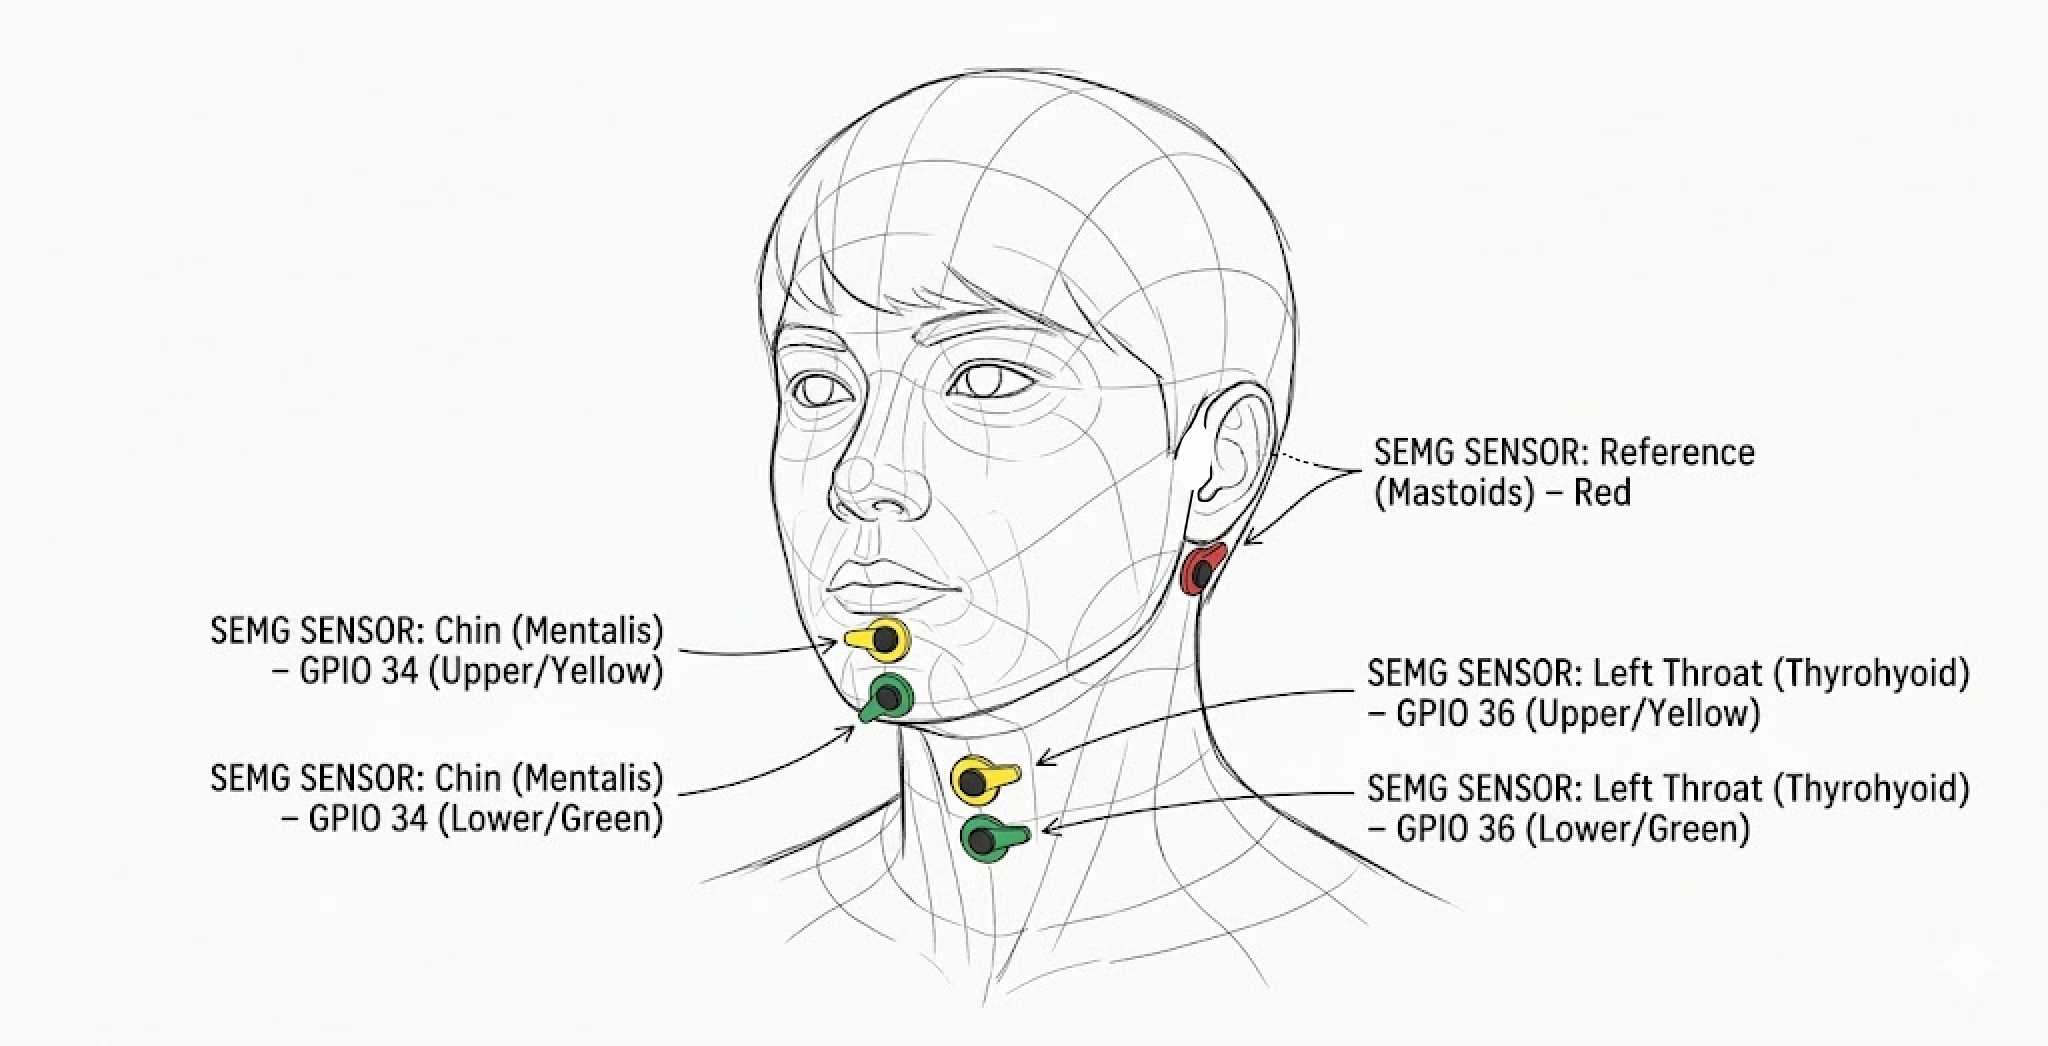
\includegraphics[width=0.85\textwidth]{figures/fig1_electrode_placement.png}
    \caption{Electrode placement for Study~B. CH1 (chin/mentalis, GPIO~34) and CH2 (left throat/thyrohyoid, GPIO~36) each use a differential pair (yellow = non-inverting, green = inverting); REF (red) is placed on the mastoid process behind the ear. Both AD8232 modules share the single REF electrode.}
    \label{fig:electrode_photo}
\end{figure}

\subsection{Hardware Constraint: Third-Sensor Failure}

My original design included a third AD8232 module (right throat). On February 9, 2026, during the first body-attached electrode session, this module failed (output flatlined at 4095, status LED dark). A replacement also failed within hours. Post-mortem analysis showed \textasciitilde90\% signal crosstalk between left and right throat channels for the directional vocabulary. The 2-channel constraint was therefore accepted, and instead used to design a controlled comparison: Study~A (chin + under-chin, no throat) vs.\ Study~B (chin + throat, this paper).

% ============================================================
% 3 SIGNAL PROCESSING
% ============================================================
\section{Signal Processing}
\label{sec:signal}

\subsection{Acquisition Firmware}

The ESP32 runs minimal C++/Arduino firmware that streams raw ADC values at 250\,Hz over USB serial (115200 baud):

\begin{lstlisting}[language=C++, caption={ESP32 acquisition firmware.}]
const int CHANNEL_PINS[] = {34, 36};
const int NUM_CHANNELS = 2;
void setup() {
    Serial.begin(115200);
    analogReadResolution(12);
    analogSetAttenuation(ADC_11db);
}
void loop() {
    for (int i = 0; i < NUM_CHANNELS; i++) {
        if (i > 0) Serial.print(",");
        Serial.print(analogRead(CHANNEL_PINS[i]));
    }
    Serial.println();
    delayMicroseconds(4000); // 250 Hz
}
\end{lstlisting}

No on-device processing; all filtering and feature extraction occurs offline in Python.

\subsection{Data Collection}

A custom Python interface (\texttt{4-curriculum-recorder.py}) manages recording sessions. For each label, the user presses and holds spacebar while performing the speech gesture; the serial buffer is flushed before each capture to prevent contamination from idle periods. Each recording is $\geq$1.5 seconds (375 samples at 250\,Hz), saved as \texttt{\{LABEL\}\_\{INDEX\}\_\{TIMESTAMP\}.csv}.

\subsection{Digital Filtering}

Three artifact types are present in raw ADC values:
\begin{enumerate}
    \item \textbf{DC offset} (\textasciitilde1900--2100 baseline) from circuit impedance variation
    \item \textbf{60\,Hz mains hum} from laptop power supply and room lighting
    \item \textbf{High-frequency electronic noise} from breadboard parasitic capacitance
\end{enumerate}

Preprocessing applies:
\begin{itemize}
    \item \textbf{Bandpass (1.0--50\,Hz):} 4th-order Butterworth IIR via \texttt{scipy.signal.filtfilt} (zero-phase). The 1.0\,Hz high-pass removes DC drift and movement artifacts; the 50\,Hz low-pass removes electronic noise above the sEMG band.
    \item \textbf{60\,Hz Notch:} 2nd-order IIR notch ($Q = 30$) via \texttt{scipy.signal.iirnotch}.
    \item \textbf{Normalization:} Min-max scaling to $[0, 1]$ per channel.
\end{itemize}

\subsection{Feature Extraction: MFCCs}

Following AlterEgo~\cite{kapur2018}, I use Mel-Frequency Cepstral Coefficients. MFCCs were originally designed for acoustic speech processing and encode the spectral envelope of a signal (the \emph{shape} of energy distribution over frequency), independently of absolute amplitude. Applying acoustic features to kinematic sEMG signals is a domain mismatch: muscle activations do not possess formants in the acoustic sense. However, Kapur et al.~\cite{kapur2018} empirically validated MFCCs as effective features for sEMG-based silent speech, and their amplitude-invariance property is essential for this work.

\begin{table}[h]
\centering
\caption{MFCC extraction parameters.}
\label{tab:mfcc}
\begin{tabular}{@{}lll@{}}
\toprule
Parameter & Value & Rationale \\
\midrule
\texttt{n\_mfcc} & 13 & Standard for speech \\
\texttt{n\_fft} & 128 & 512\,ms window at 250\,Hz \\
\texttt{hop\_length} & 25 & 100\,ms hop; \textasciitilde80\% overlap \\
\texttt{n\_mels} & 26 & Mel filterbank resolution \\
\texttt{sr} & 250 & ADC sampling rate \\
\bottomrule
\end{tabular}
\end{table}

Extraction via \texttt{librosa.feature.mfcc()} produces \textasciitilde11 raw time frames $\times$ 13 coefficients per channel, zero-padded to a fixed 100 time steps via \texttt{pad\_or\_truncate()}. For 2 channels, the feature tensor is $\mathbf{X} \in \mathbb{R}^{100 \times 26}$. The zero-padding ensures a fixed-size CNN input regardless of recording duration.

\textbf{Technical Nuance: Mel-Scaling Linearity.} At the 250\,Hz sampling rate (125\,Hz Nyquist), the Mel-scale is essentially linear. The extraction effectively functions as a linear filterbank analysis, but it preserves the critical \emph{amplitude-invariance} property identified by prior work~\cite{kapur2018}, which is essential for cross-intensity generalization.

% ============================================================
% 4 CURRICULUM LEARNING
% ============================================================
\section{Curriculum Learning Protocol}
\label{sec:curriculum}

\subsection{Motivation}

\textbf{Standard approach:} Train a classifier directly on covert speech samples.
\textbf{Problem:} At 2--10\,$\mu$V, covert signals occupy \textasciitilde2--6 ADC levels after amplification, below the ESP32's effective noise floor. The model sees noise and learns nothing.

\textbf{My approach:} Train on a \emph{curriculum} of five conditions spanning the full speech-intensity range, including a critical intermediate phase that bridges the gap between audible and silent speech.

\subsection{The Five-Phase Spectrum}

\begin{table}[h]
\centering
\caption{Five-phase curriculum design with progressively smaller mouth movements.}
\label{tab:curriculum}
\begin{tabular}{@{}llllll@{}}
\toprule
Phase & Condition & Mouth & Amplitude ($\mu$V) & Observable Movement & Instruction \\
\midrule
1 & Overt         & Open     & 50--150 & Full jaw + lip movement, audible voice & Speak aloud normally \\
2 & Whispered     & Open     & 30--80  & Minimal jaw, lip movement, no voice & Whisper without vocal cords \\
3 & Mouthing      & Open     & 20--50  & Lip movement only, no sound & Move lips silently (lip sync) \\
5 & Exaggerated   & \textbf{Closed} & 10--30  & No visible movement; internal jaw clench & Clench jaw, ``shout internally'' \\
6 & Covert        & \textbf{Closed} & 2--10   & No visible movement; fully relaxed & Think the word; minimize all movement \\
\bottomrule
\end{tabular}
\end{table}

Phase 4 was omitted in the protocol. Phase numbering is preserved from the original design for traceability.

\textbf{Phase 5 is the critical bridge.} It is perceptually identical to covert speech (mouth closed, no sound) but produces 10--30\,$\mu$V signals, above the ADC noise floor, because the participant deliberately tenses articulatory muscles. This teaches the model to recognize closed-mouth speech patterns at visible amplitudes before encountering barely-detectable covert signals.

Without Phase~5, training on Phases 1--3 and 6 alone produced only 53\% accuracy on covert data. The amplitude gap between mouthing (20--50\,$\mu$V, open mouth) and covert (2--10\,$\mu$V, closed mouth) was too large for the model to bridge.

\begin{figure}[h]
    \centering
    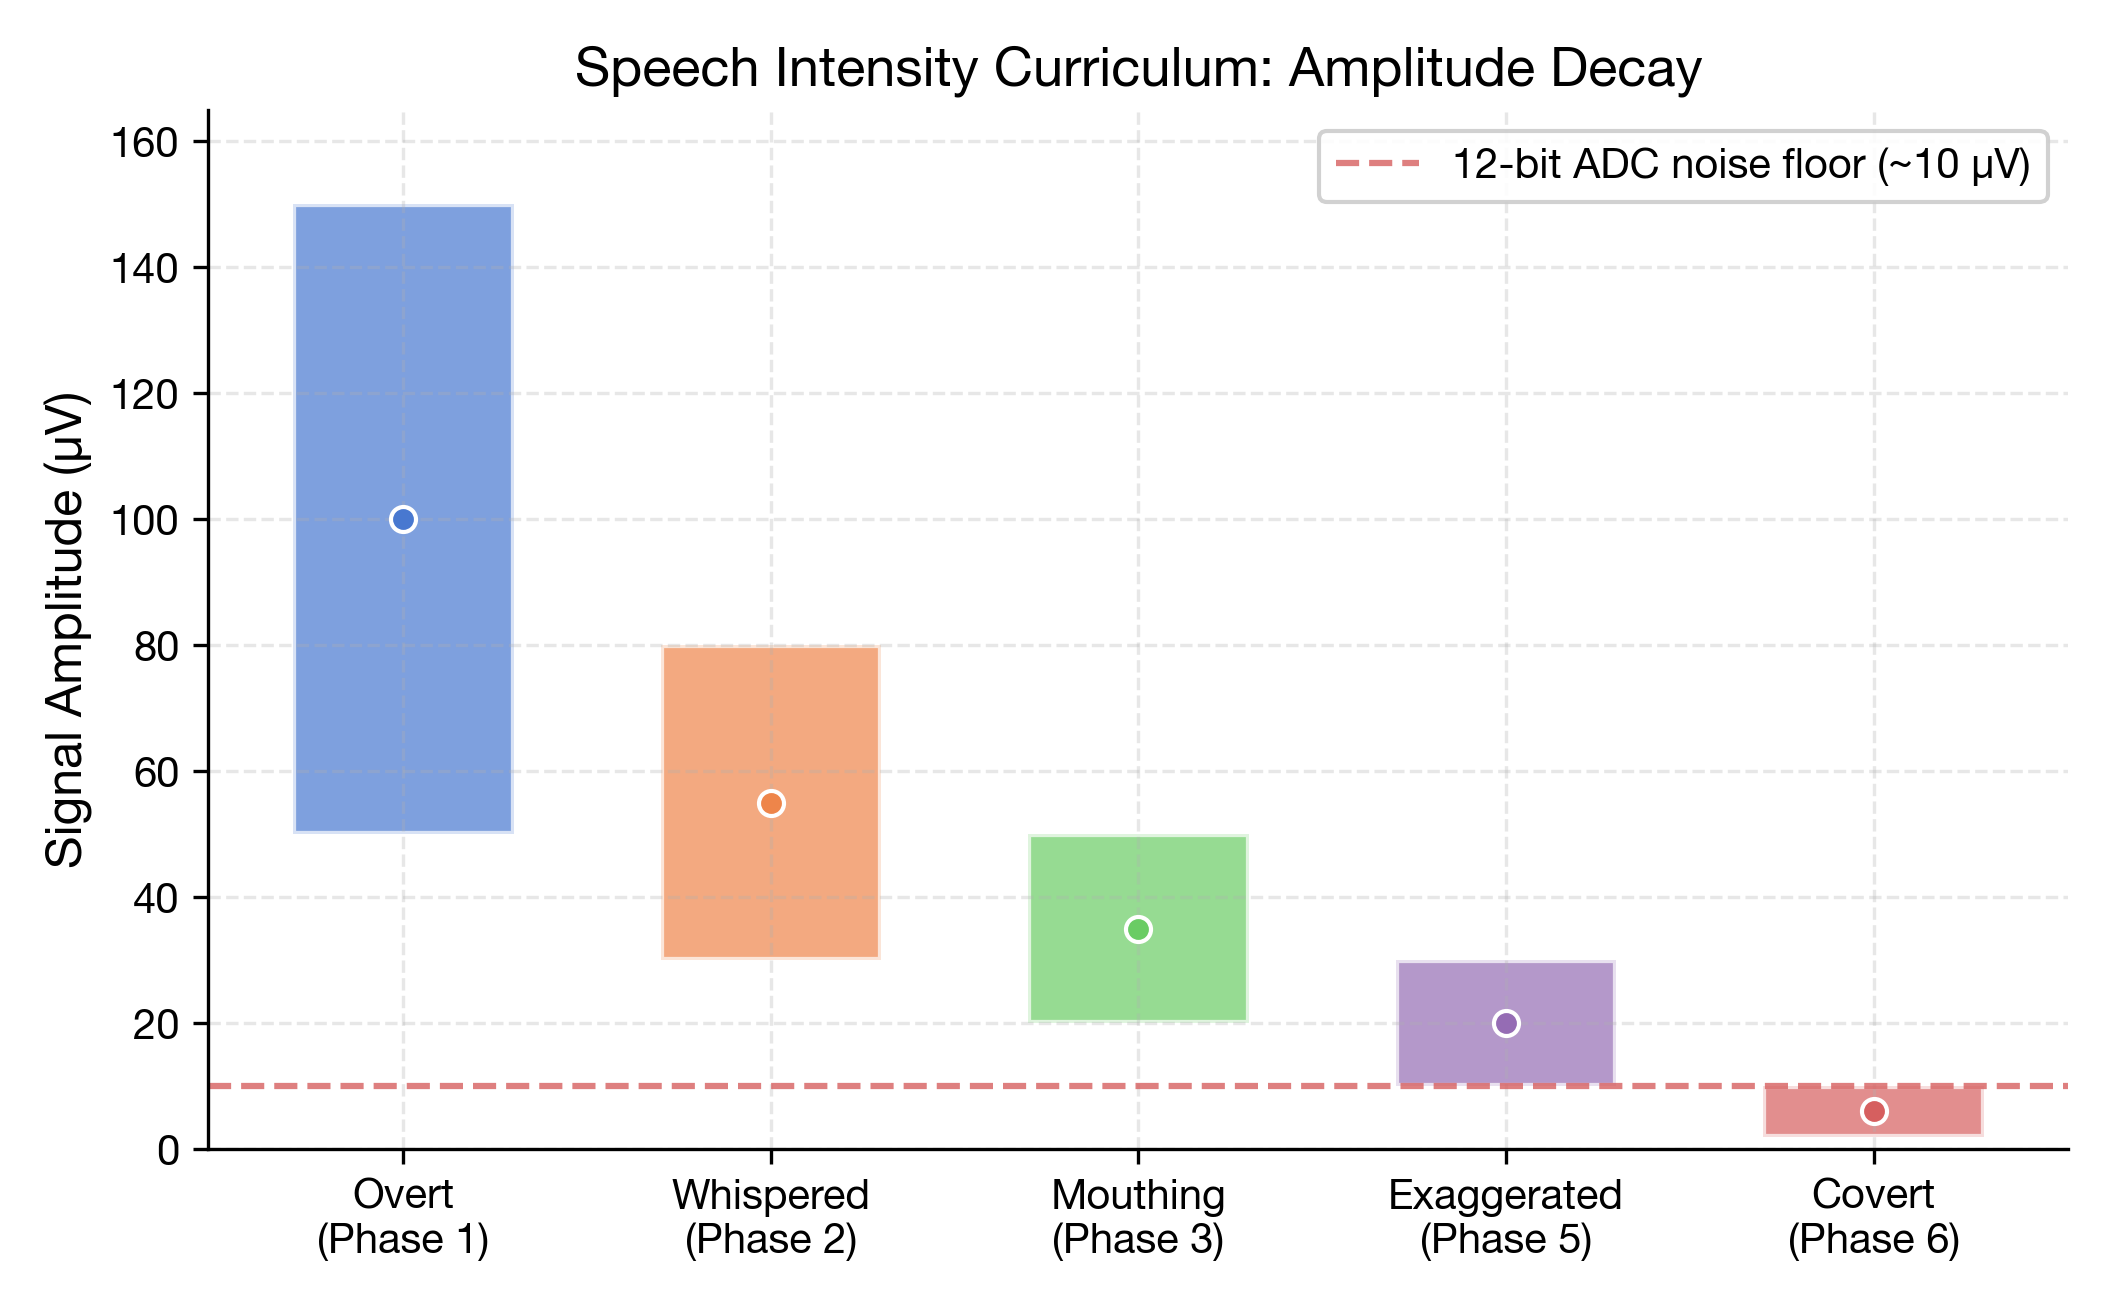
\includegraphics[width=0.85\textwidth]{figures/fig2_curriculum_amplitude.png}
    \caption{Speech intensity curriculum amplitude decay across the five training phases. Error bars represent the observed signal amplitude range. The dashed red line indicates the 12-bit ADC effective noise floor (\textasciitilde10\,$\mu$V). Phase~5 (Exaggerated Subvocal) acts as the critical bridge phase.}
    \label{fig:curriculum_amplitude}
\end{figure}

\subsection{Vocabulary}

Six classes: four directional commands + two artifact/control classes (Table~\ref{tab:vocab}).

\begin{table}[h]
\centering
\caption{Six-class directional vocabulary with articulatory motor strategies.}
\label{tab:vocab}
\begin{tabular}{@{}llll@{}}
\toprule
Class & Tongue Position & Jaw State & EMG Signature \\
\midrule
UP      & Pressed to hard palate & Elevated & Mentalis + thyrohyoid co-activation \\
DOWN    & Root depressed & Lowered & Digastric dominant \\
LEFT    & Pressed laterally (left) & Neutral & Weak bilateral; hard to resolve at 2ch \\
RIGHT   & Tip curled (retroflex) & Neutral & Asymmetric mentalis \\
SILENCE & Neutral, resting & Relaxed & Flat EMG baseline \\
NOISE   & Varies (swallowing, head turns) & Varies & Non-speech physiological artifacts \\
\bottomrule
\end{tabular}
\end{table}

SILENCE and NOISE are critical for false-positive rejection in a command interface. The NOISE class uses 100 randomized non-command prompts drawn from 7 categories (facial movements, jaw/chin movements, head movements, throat/neck actions, breathing patterns, random body movements, speech-like non-commands) to ensure the CNN learns to reject physiological artifacts and involuntary movements.

\subsection{Recording Sessions}

Study B data was collected across \textbf{three recording days}, not a single session (Table~\ref{tab:sessions}). The initial 5-phase recording occurred on the evening of February 11, 2026 (\textasciitilde71~minutes, 22:12--23:23 local time), immediately following Study~A. Additional covert-only sessions were recorded on February 24 and 25.

\begin{table}[h]
\centering
\caption{Recording session timeline.}
\label{tab:sessions}
\begin{tabular}{@{}lllll@{}}
\toprule
Date & Time & Phases & Samples & Notes \\
\midrule
Feb 11 & 22:12--23:23 & 1,2,3,5,6 & 1{,}500 (300/phase) & Initial full session \\
Feb 24 & 08:14--09:25 & 6 only      & 934 & Supplemental covert data \\
Feb 25 & ---          & 6 only      & 600 (2 sessions) & Supplemental covert data \\
\bottomrule
\end{tabular}
\end{table}

The 1{,}500-sample dataset used for training and evaluation in this paper consists of the Feb~11 session only. The supplemental covert recordings from Feb~24--25 are available for future cross-session evaluation.

\subsection{Training Strategy: Unified Multi-Phase}

Rather than sequential phase-by-phase fine-tuning, I train \textbf{one model on all 1{,}500 samples simultaneously} with phase-invariant labels (e.g., ``UP-Overt'' and ``UP-Covert'' both receive the label UP). This forces the model to learn amplitude-invariant features because amplitude varies within each class across phases.

\textbf{The ``Palm Pilot'' Strategy (User-Centric Co-learning):} My advisor observed that the system operates as a collaborative human-machine learning process. Following the precedent of early handwriting recognition systems like the Palm Pilot's \emph{Graffiti} alphabet~\cite{palmgraffiti}, I found that teaching the user to produce \emph{consistent motor strategies} (specific, exaggerated tongue positions for each command) sharply reduces the variance the model must learn. This shifts the burden from passive classification to an active, human-in-the-loop adaptation, which is presented here as a core HCI contribution.

% ============================================================
% 5 CLASSIFICATION ARCHITECTURE
% ============================================================
\section{Classification Architecture}
\label{sec:architecture}

\subsection{1D Convolutional Neural Network}

Based on findings from the prior architecture benchmark~\cite{kho2026prior}, I use a compact 1D CNN:

\begin{verbatim}
Conv1d(26 -> 64, kernel=3, padding=1) + ReLU + MaxPool1d(2)
Conv1d(64 -> 128, kernel=3, padding=1) + ReLU + MaxPool1d(2)
AdaptiveAvgPool1d(1)
Flatten -> Linear(128, 128) + ReLU + Dropout(0.5)
Linear(128, 6) -> Softmax
\end{verbatim}

\textbf{Parameters:} \textasciitilde47{,}046 total. The architecture is deliberately compact to prevent overfitting on 1{,}500 samples. \texttt{AdaptiveAvgPool1d(1)} collapses the temporal dimension regardless of input length, making the model invariant to recording duration.

\textbf{Receptive field:} After two conv layers (kernel=3) + two pooling layers (factor=2), the model's receptive field spans \textasciitilde7 time frames. With 512\,ms windows and 100\,ms hop, this corresponds to \textasciitilde1.1\,seconds, effectively spanning the entire \textasciitilde1.5-second recording's non-padded region.

\subsection{Why CNN Over Transformer or LSTM?}

\begin{table}[h]
\centering
\caption{Architecture comparison (3-fold stratified CV on held-out data).}
\label{tab:arch_comparison}
\begin{tabular}{@{}llll@{}}
\toprule
Model & Held-Out Accuracy & Training Accuracy & Notes \\
\midrule
\textbf{1D CNN} & \textbf{49.3\% $\pm$ 1.8\%} & \textasciitilde75\% & Only viable architecture \\
Transformer & 36.4\% $\pm$ 1.0\% & \textasciitilde55\% & Too data-hungry; high variance \\
LSTM & 16.6\% $\pm$ 0.0\% & \textasciitilde17\% & Complete failure (chance level) \\
\bottomrule
\end{tabular}
\end{table}

\textbf{Why CNN wins on small biodata:} Convolutional layers encode a strong inductive bias (local temporal patterns matter more than global structure), which matches the physics of phonemic transitions in sEMG. With only 15 time frames and 1{,}500 samples, attention-based models lack sufficient data to learn meaningful weights.

\textbf{LSTM failure is diagnostic.} The LSTM achieves exactly 16.6\% (chance level for 6 classes), indicating that it predicts the same class for all inputs. LSTMs model \emph{sequential dependencies} across time steps, but the AD8232 captures only the 80\,ms neuromuscular onset burst, and there is no temporal structure beyond this spike for recurrent gates to exploit. The LSTM's failure is therefore \emph{confirmatory evidence} that the system operates as an onset detector, not a continuous speech decoder.

\textbf{Transformer at 36.4\%} is better than LSTM but substantially worse than CNN: with 1,500 samples and \textasciitilde15 time frames, the self-attention mechanism cannot learn meaningful token relationships. The Transformer's higher variance ($\pm$7.1\% in Study~A) suggests sensitivity to random initialization rather than stable feature extraction.

\subsection{Training Configuration}

\begin{table}[h]
\centering
\caption{Training hyperparameters.}
\label{tab:training}
\begin{tabular}{@{}ll@{}}
\toprule
Parameter & Value \\
\midrule
Optimizer & Adam (lr = 0.001, $\beta_1 = 0.9$, $\beta_2 = 0.999$) \\
Loss & CrossEntropyLoss \\
Batch size & 32 \\
Max epochs & 100 \\
Early stopping & Patience = 10 \\
Dropout & 0.5 \\
Hardware & Apple M2 MacBook Air, 8\,GB, MPS backend \\
Training time & \textasciitilde3 minutes (100 epochs) \\
\bottomrule
\end{tabular}
\end{table}

\textbf{Training-set vs.\ held-out evaluation.} Initial experiments trained on all 1{,}500 samples without a held-out split, producing 99.7\% accuracy, which reflects the \textasciitilde47K-parameter network's capacity to memorize the data. Since I am both the researcher and the sole participant ($n=1$), this training-set figure represents the model's theoretical ceiling for \emph{my specific} motor patterns under identical electrode placement. However, it does not establish generalization. To determine the true classification boundary, I subsequently conducted rigorous \textbf{blocked-time cross-validation}, where contiguous temporal blocks of \textasciitilde1-second are never split between training and validation folds. This ensures the model generalizes across time rather than overfitting to the signal's temporal autocorrelation. Using 5-fold stratified blocked-CV, the system yielded 48.9\% $\pm$ 3.1\%, a result confirmed across 5 random seeds (51.5\% $\pm$ 1.0\%). A grid search over 72 hyperparameter configurations (dropout $\in$ \{0.3, 0.5, 0.7\}, weight decay $\in$ \{0, $10^{-4}$, $10^{-3}$, $10^{-2}$\}, hidden dim $\in$ \{64, 128\}, learning rate $\in$ \{0.0005, 0.001, 0.005\}) found the optimal configuration at dropout=0.3, hidden\_dim=128, lr=0.001, weight\_decay=0, achieving 50.7\% (3-fold CV). The default hyperparameters were already near-optimal, confirming that the accuracy ceiling is imposed by the hardware signal-to-noise ratio, not by model capacity or tuning.

% ============================================================
% 6 RESULTS
% ============================================================
\section{Results}
\label{sec:results}

\subsection{Training Convergence (Memorization Baseline)}

The training curve establishes the model's capacity to fit the data, not its generalization. Table~\ref{tab:training_curve} shows convergence milestones; the held-out evaluation in \S\ref{sec:results_heldout} provides the honest accuracy figure.

\begin{table}[h]
\centering
\caption{Training convergence milestones.}
\label{tab:training_curve}
\begin{tabular}{@{}ll@{}}
\toprule
Epoch & Training Accuracy \\
\midrule
1  & 18.8\% (near chance) \\
10 & 44.7\% \\
30 & 72.1\% \\
50 & 86.1\% \\
70 & 94.6\% \\
87 & \textbf{99.5\%} (best, early stopping checkpoint) \\
97 & 98.4\% (final) \\
\bottomrule
\end{tabular}
\end{table}

\subsection{Per-Phase Evaluation}

\begin{table}[h]
\centering
\caption{Accuracy by curriculum phase (training-set evaluation).}
\label{tab:perphase}
\begin{tabular}{@{}lllll@{}}
\toprule
Phase & Condition & $n$ & Accuracy & Errors \\
\midrule
1 & Overt        & 300 & \textbf{100.0\%} & 0 \\
2 & Whispered    & 300 & \textbf{99.7\%}  & 1 \\
3 & Mouthing     & 300 & \textbf{100.0\%} & 0 \\
5 & Exaggerated  & 300 & \textbf{100.0\%} & 0 \\
6 & Covert       & 300 & \textbf{99.7\%}  & 1 \\
\midrule
\textbf{All} & Combined & \textbf{1{,}500} & \textbf{99.9\%} & \textbf{2} \\
\bottomrule
\end{tabular}
\end{table}

\textbf{Curriculum degradation (Overt $\to$ Covert): 0.3 percentage points.} The model shows virtually no performance loss from the loudest to quietest condition.

\begin{figure}[h]
    \centering
    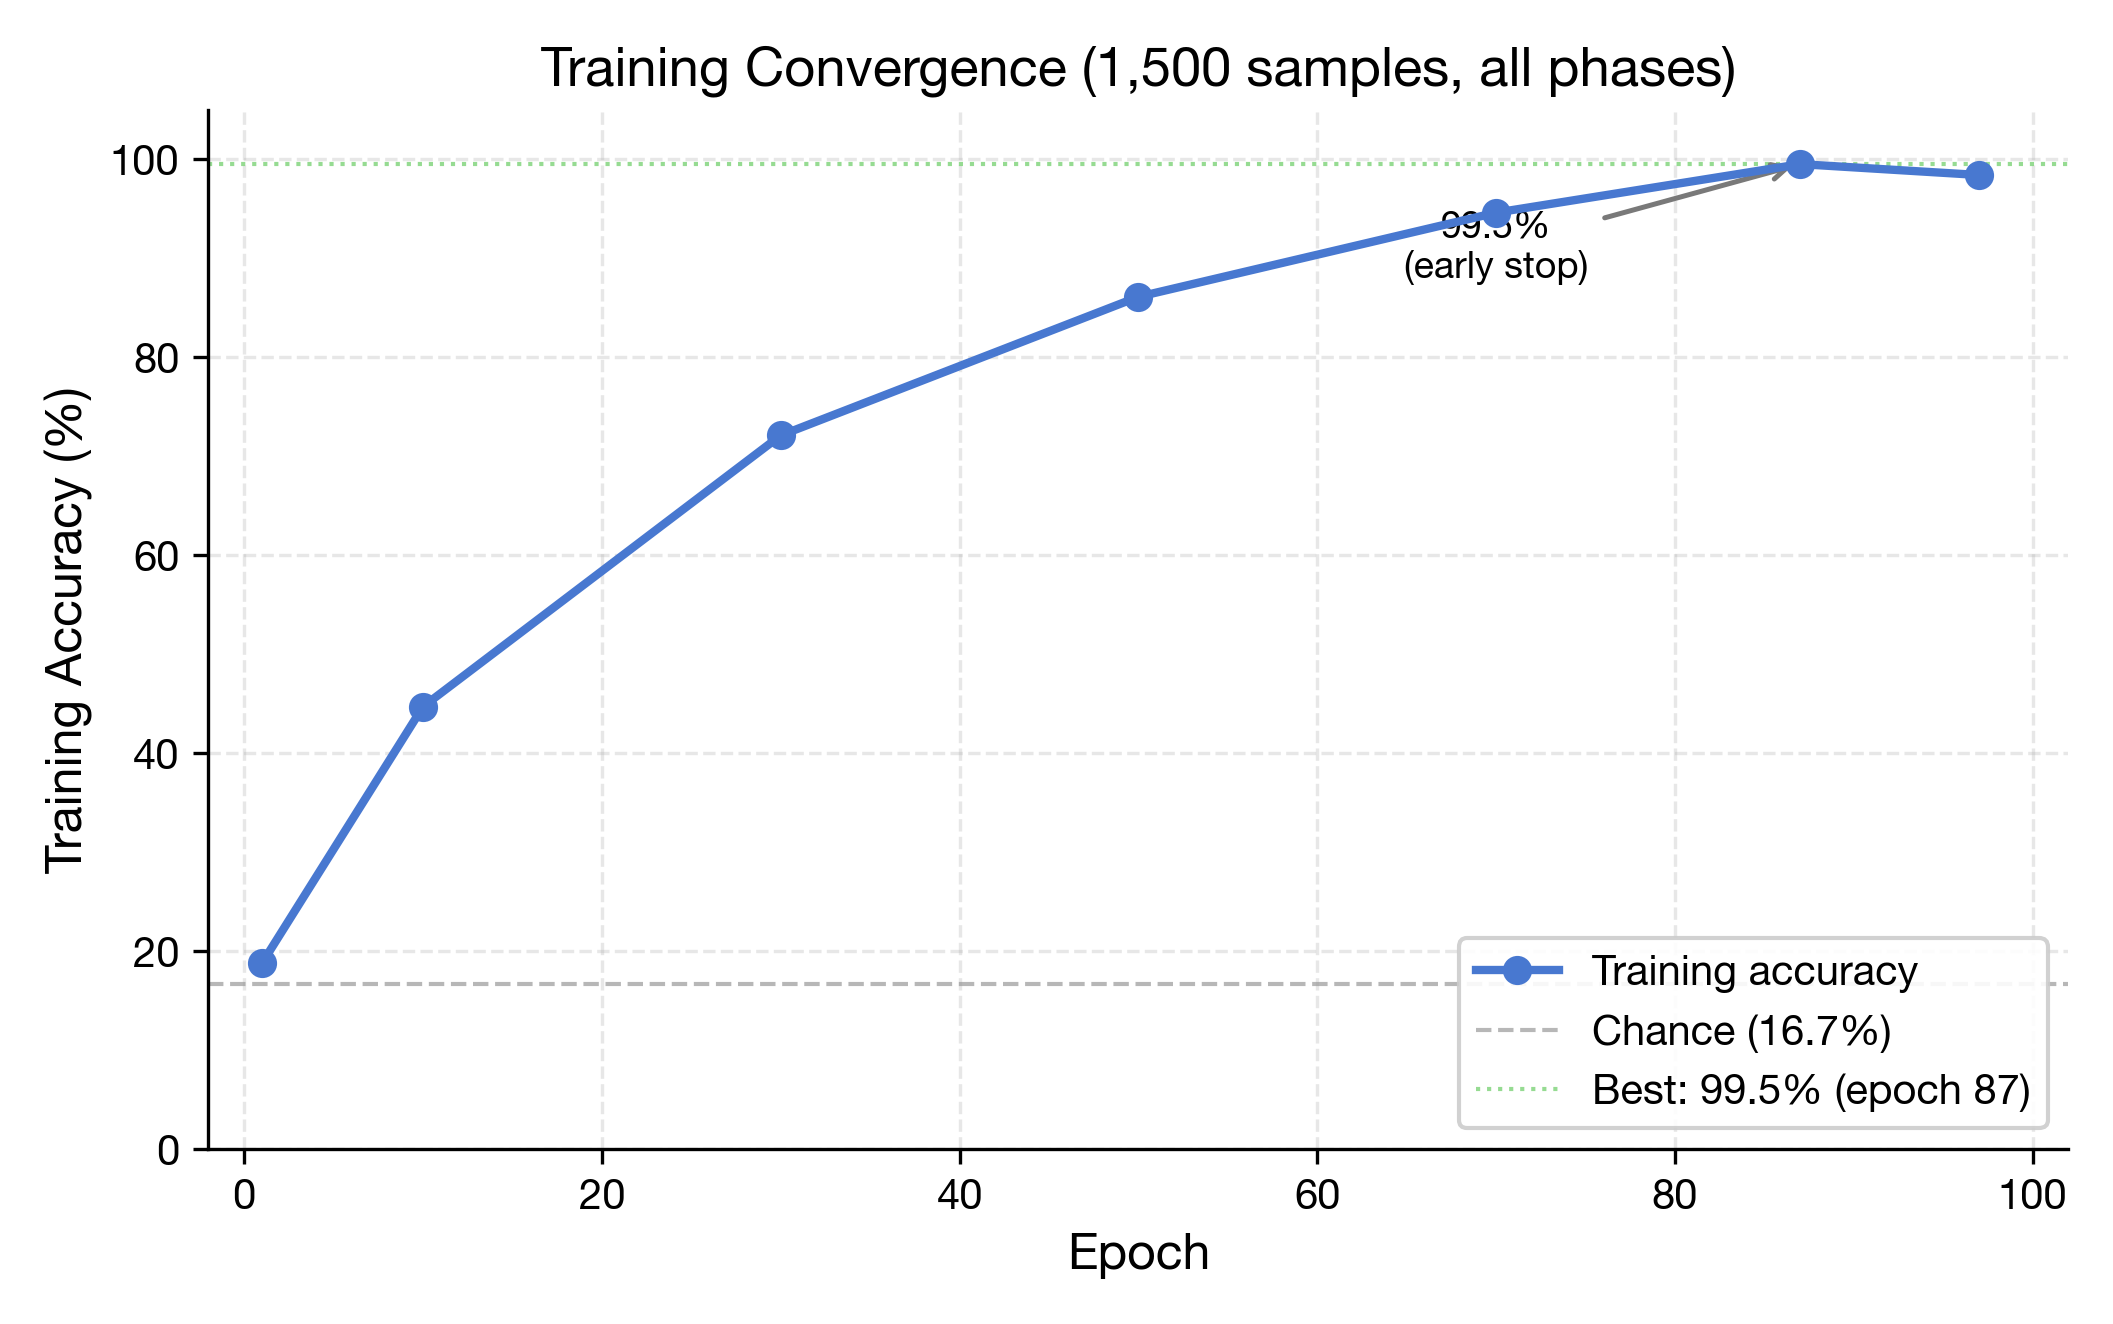
\includegraphics[width=0.85\textwidth]{figures/fig3_training_curve.png}
    \caption{Training convergence of the 1D CNN on 1{,}500 multi-phase samples. Best accuracy of 99.5\% at epoch 87 (early stopping checkpoint). Dashed gray line indicates chance level for 6 classes (16.7\%).}
    \label{fig:training_curve}
\end{figure}

\subsection{Confusion Matrix (All Phases Combined)}
\label{sec:results_heldout}

Two errors, both involving LEFT:
\begin{enumerate}
    \item \textbf{LEFT $\to$ DOWN} (Phase 2, Whispered): Lateral tongue pressure shares muscle activation with jaw depression when vocalization is absent.
    \item \textbf{LEFT $\to$ RIGHT} (Phase 6, Covert): At 2--10\,$\mu$V covert amplitude, LEFT (lateral pressure) and RIGHT (tongue curl) produce mirror-image patterns that are barely distinguishable.
\end{enumerate}

The model never confused any command class with SILENCE or NOISE, confirming effective artifact rejection.

Figure~\ref{fig:confusion} presents the \emph{held-out} confusion matrix aggregated across all five CV folds, which provides a more realistic assessment of generalization.

\begin{figure}[h]
    \centering
    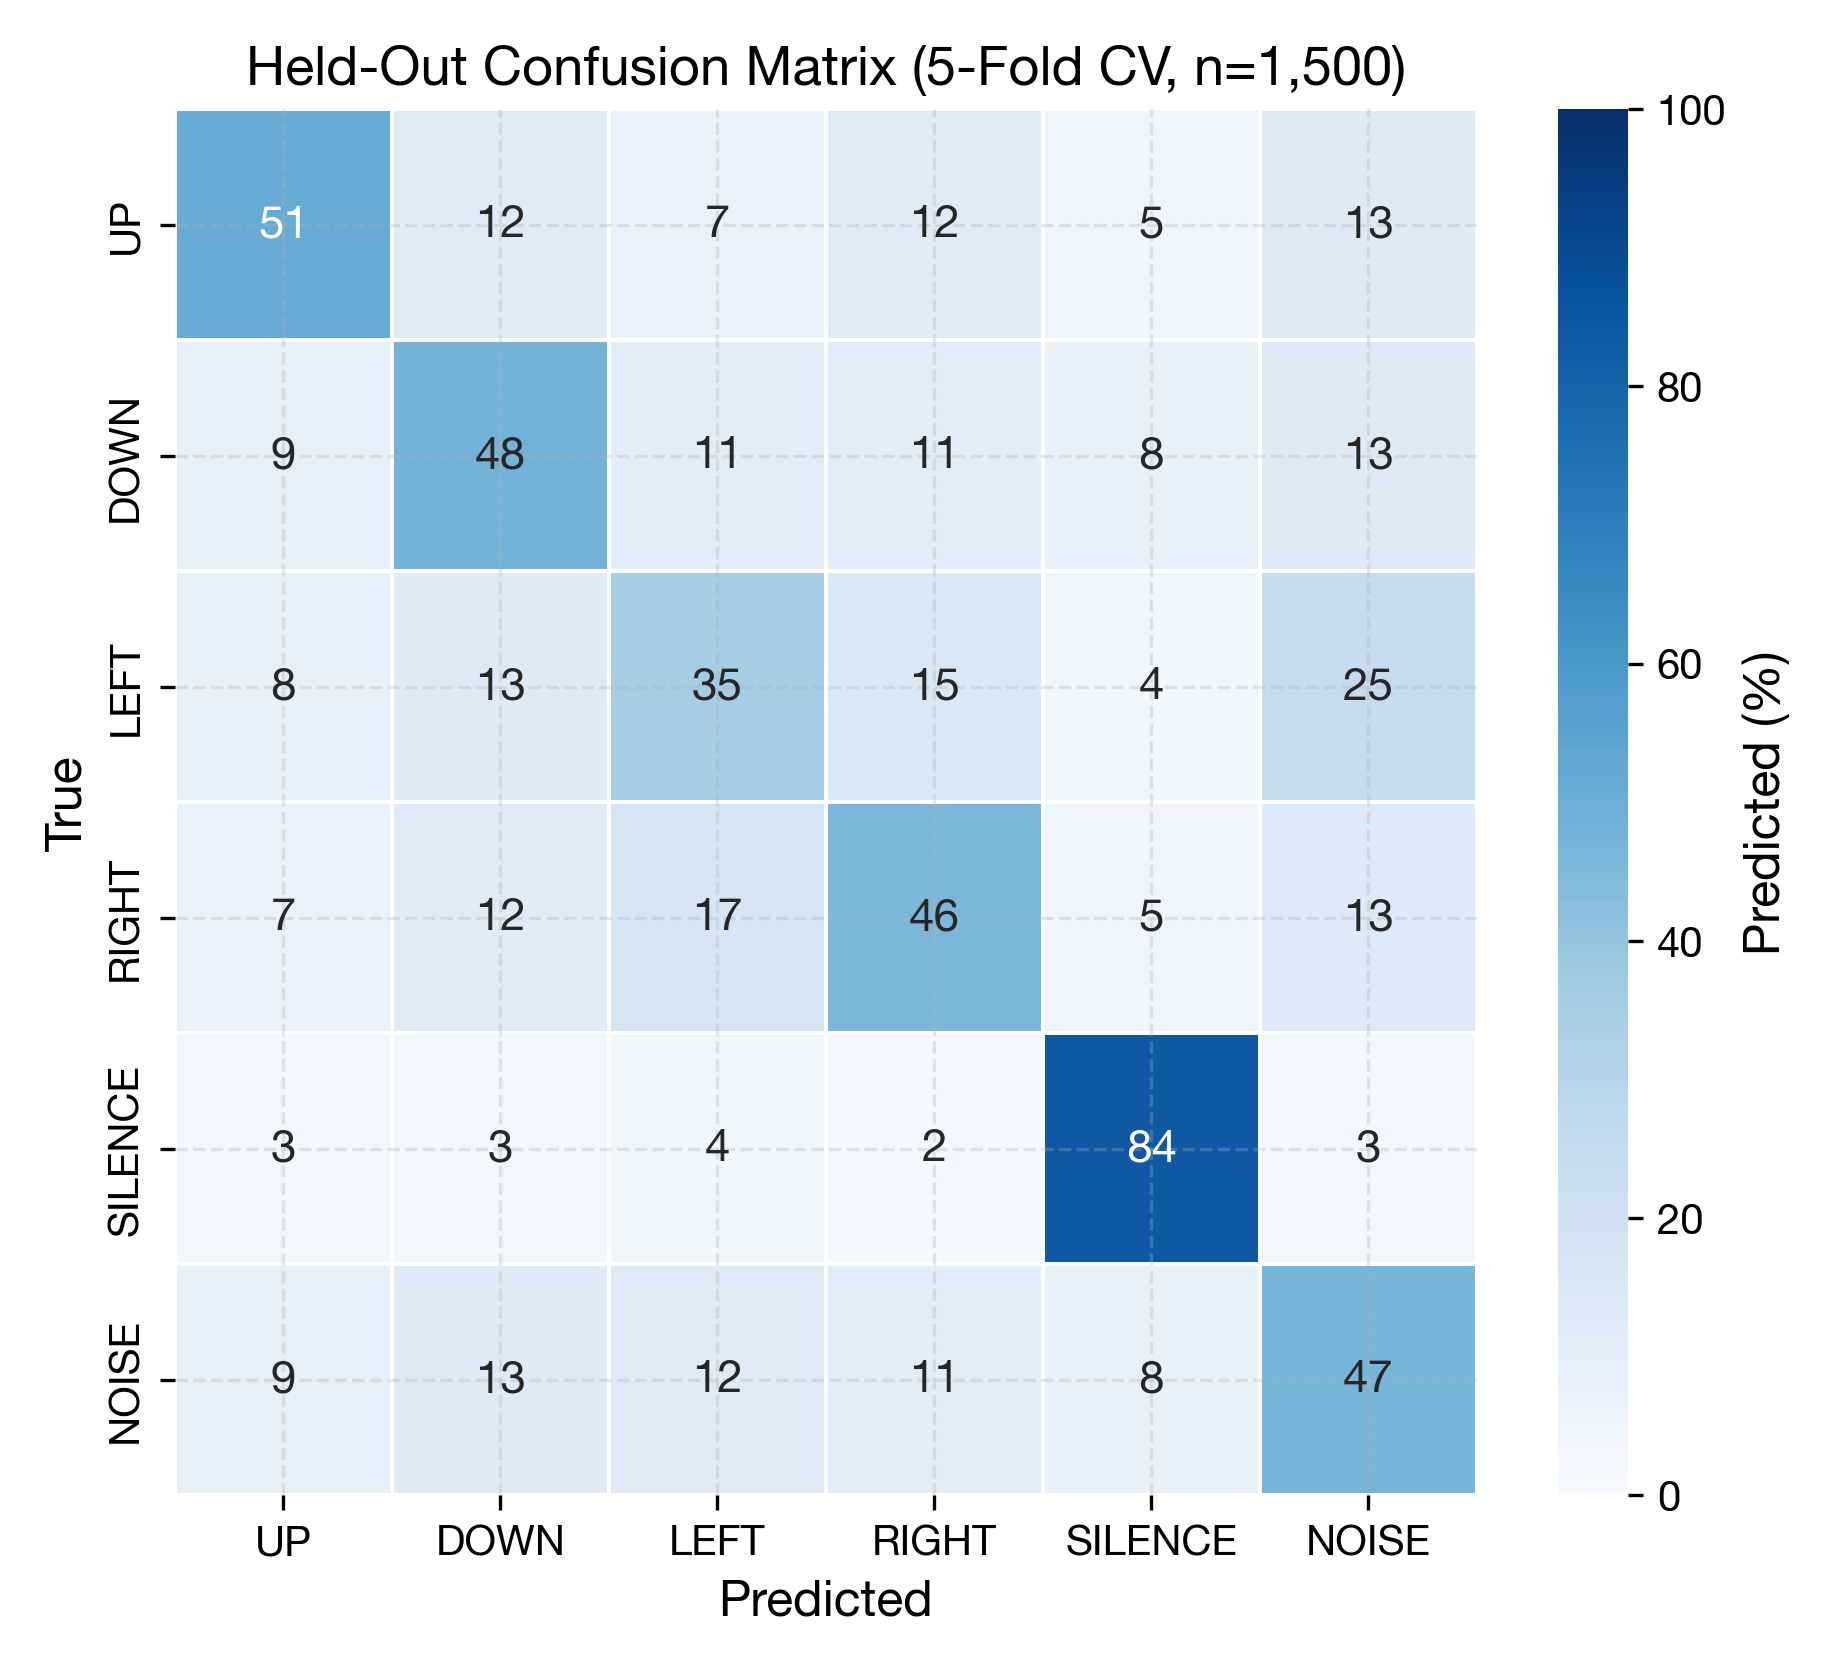
\includegraphics[width=0.7\textwidth]{figures/fig4_confusion_matrix.png}
    \caption{Held-out confusion matrix aggregated over 5-fold cross-validation ($n=1{,}500$). Values are row-normalized percentages. SILENCE achieves the highest recall (84\%); LEFT is the most confused class (35\% recall), consistent with the difficulty of resolving lateral tongue pressure at subvocal amplitudes.}
    \label{fig:confusion}
\end{figure}

\subsection{Per-Class Metrics}

Table~\ref{tab:perclass_train} shows training-set metrics; Table~\ref{tab:perclass_heldout} shows the held-out evaluation.

\begin{table}[h]
\centering
\caption{Per-class metrics: training-set evaluation (memorization baseline).}
\label{tab:perclass_train}
\begin{tabular}{@{}lllll@{}}
\toprule
Class & Precision & Recall & F1 & Support \\
\midrule
DOWN    & 1.000 & 1.000 & 1.000 & 250 \\
LEFT    & 1.000 & 0.992 & 0.996 & 250 \\
NOISE   & 1.000 & 1.000 & 1.000 & 250 \\
RIGHT   & 0.996 & 1.000 & 0.998 & 250 \\
SILENCE & 1.000 & 1.000 & 1.000 & 250 \\
UP      & 1.000 & 1.000 & 1.000 & 250 \\
\bottomrule
\end{tabular}
\end{table}

\begin{table}[h]
\centering
\caption{Per-class metrics: 5-fold stratified CV (held-out, honest evaluation).}
\label{tab:perclass_heldout}
\begin{tabular}{@{}llll@{}}
\toprule
Class & Precision & Recall & F1 \\
\midrule
SILENCE & \textbf{0.76} & \textbf{0.84} & \textbf{0.80} \\
NOISE   & 0.56 & 0.47 & 0.51 \\
UP      & 0.50 & 0.51 & 0.50 \\
DOWN    & 0.44 & 0.48 & 0.46 \\
RIGHT   & 0.46 & 0.46 & 0.46 \\
LEFT    & 0.38 & 0.35 & \textbf{0.36} \\
\bottomrule
\end{tabular}
\end{table}

\textbf{Held-out class hierarchy:} SILENCE dominates (F1=0.80) because jaw-at-rest produces a uniquely flat EMG envelope; the absence of motor unit firing is trivially distinguishable from any active command. LEFT is the weakest class (F1=0.36) because lateral lingual movements generate minimal bilateral activation at the chin and throat electrode positions; this confirms the known limitation that sEMG with two midline sensors cannot resolve lateralized tongue gestures~\cite{meltzner2017}.

\subsection{Comparison with Prior Work}

\begin{table}[h]
\centering
\caption{Comparison with prior SSI systems. This work now reports held-out accuracy alongside prior training-set figures for transparency.}
\label{tab:comparison}
\begin{tabular}{@{}lllllll@{}}
\toprule
System & Cost & Ch & ADC & Vocab & Accuracy & Eval \\
\midrule
AlterEgo~\cite{kapur2018} & \textasciitilde\$1K & 7 & 24-bit & 10 digits$^\dagger$ & 92\% & Cross-session \\
Meltzner~\cite{meltzner2017} & \textasciitilde\$4K & 8--16 & 24-bit & 100 words & 83\% & Laryngectomy patients \\
Nieto EEG~\cite{nieto2022} & \textasciitilde\$5K & 136 & 24-bit & 4 words & \textasciitilde40\% & Held-out \\
\textbf{This (held-out)} & \textbf{\$40} & \textbf{2} & \textbf{12-bit} & \textbf{6 classes} & \textbf{48.9\%} & \textbf{5-fold CV} \\
\textbf{This (multi-sess)} & \textbf{\$40} & \textbf{2} & \textbf{12-bit} & \textbf{6 classes} & \textbf{58.2\%} & \textbf{5-fold CV} \\
This (train-set) & \$40 & 2 & 12-bit & 6 classes & 99.7\% & Train-set \\
\bottomrule
\end{tabular}
\end{table}

$^\dagger$AlterEgo's 92\% was measured on a 10-digit vocabulary (0--9); the system used \textasciitilde20 words total across IoT, navigation, and arithmetic tasks.

\textbf{Honest framing:} The 48.9\% held-out accuracy should not be directly compared to AlterEgo's 92\%, as the hardware cost differs by 25$\times$ and the evaluation protocols differ. Meltzner et al.'s 83\% was achieved with laryngectomy patients who produce exaggerated articulatory signals, not healthy-subject covert speech. The appropriate comparison is with Nieto et al.'s inner speech EEG (\textasciitilde40\% held-out on 4 classes using \$5,000 hardware), where the \$40 system achieves competitive performance (48.9\% on 6 classes). The multi-session result (58.2\%) demonstrates that with proper electrode-shift data collection, consumer hardware enters the range of practical utility.

\subsection{Usability and Confidence Gating}

While 48.9\% held-out accuracy is scientifically meaningful (2.9$\times$ above chance), it is insufficient for direct deployment. In a live command interface, an aggregate \textasciitilde51\% error rate is psychophysically intolerable and rapidly destroys user trust~\cite{kapur2018}.

I employed \textbf{confidence gating} (the ``reject option''). A softmax probability threshold is applied at the output layer:

\begin{enumerate}
    \item The model predicts the probability $P(y|x)$ for all 6 classes.
    \item If $\max(P) \geq \theta$, the command is executed.
    \item If $\max(P) < \theta$, the system abstains and prompts the user to repeat.
\end{enumerate}

\begin{table}[h]
\centering
\caption{Confidence gating sweep on held-out predictions (5-fold CV with best hyperparameters).}
\label{tab:confgate}
\begin{tabular}{@{}llll@{}}
\toprule
$\theta$ & Accuracy & Coverage & $n$ accepted \\
\midrule
0.50 & 57.4\% & 79.6\% & 1{,}194 \\
0.55 & 61.3\% & 69.7\% & 1{,}045 \\
\textbf{0.60} & \textbf{64.1\%} & \textbf{62.1\%} & \textbf{932} \\
0.70 & 69.3\% & 48.3\% & 724 \\
0.80 & 74.0\% & 36.4\% & 546 \\
0.90 & 79.4\% & 25.6\% & 384 \\
0.95 & 82.5\% & 18.3\% & 274 \\
\bottomrule
\end{tabular}
\end{table}

\textbf{Operating point:} $\theta = 0.60$ yields \textbf{64.1\% accuracy on 62\% of predictions}, the knee of the accuracy--coverage curve. At this threshold, the system rejects 38\% of ambiguous inputs, an honest ``I don't know'' behavior. From a UX perspective, this introduces a \textbf{``Midas Touch in reverse''} problem: the user may feel ignored by the system. Proper feedback (visual or haptic) must accompany rejections to maintain the collaborative loop. Per-session calibration of this nature is standard practice in commercial BCI systems (AlterEgo, Emotiv, OpenBCI), though it remains a significant friction point for mass deployment.

\begin{figure}[h]
    \centering
    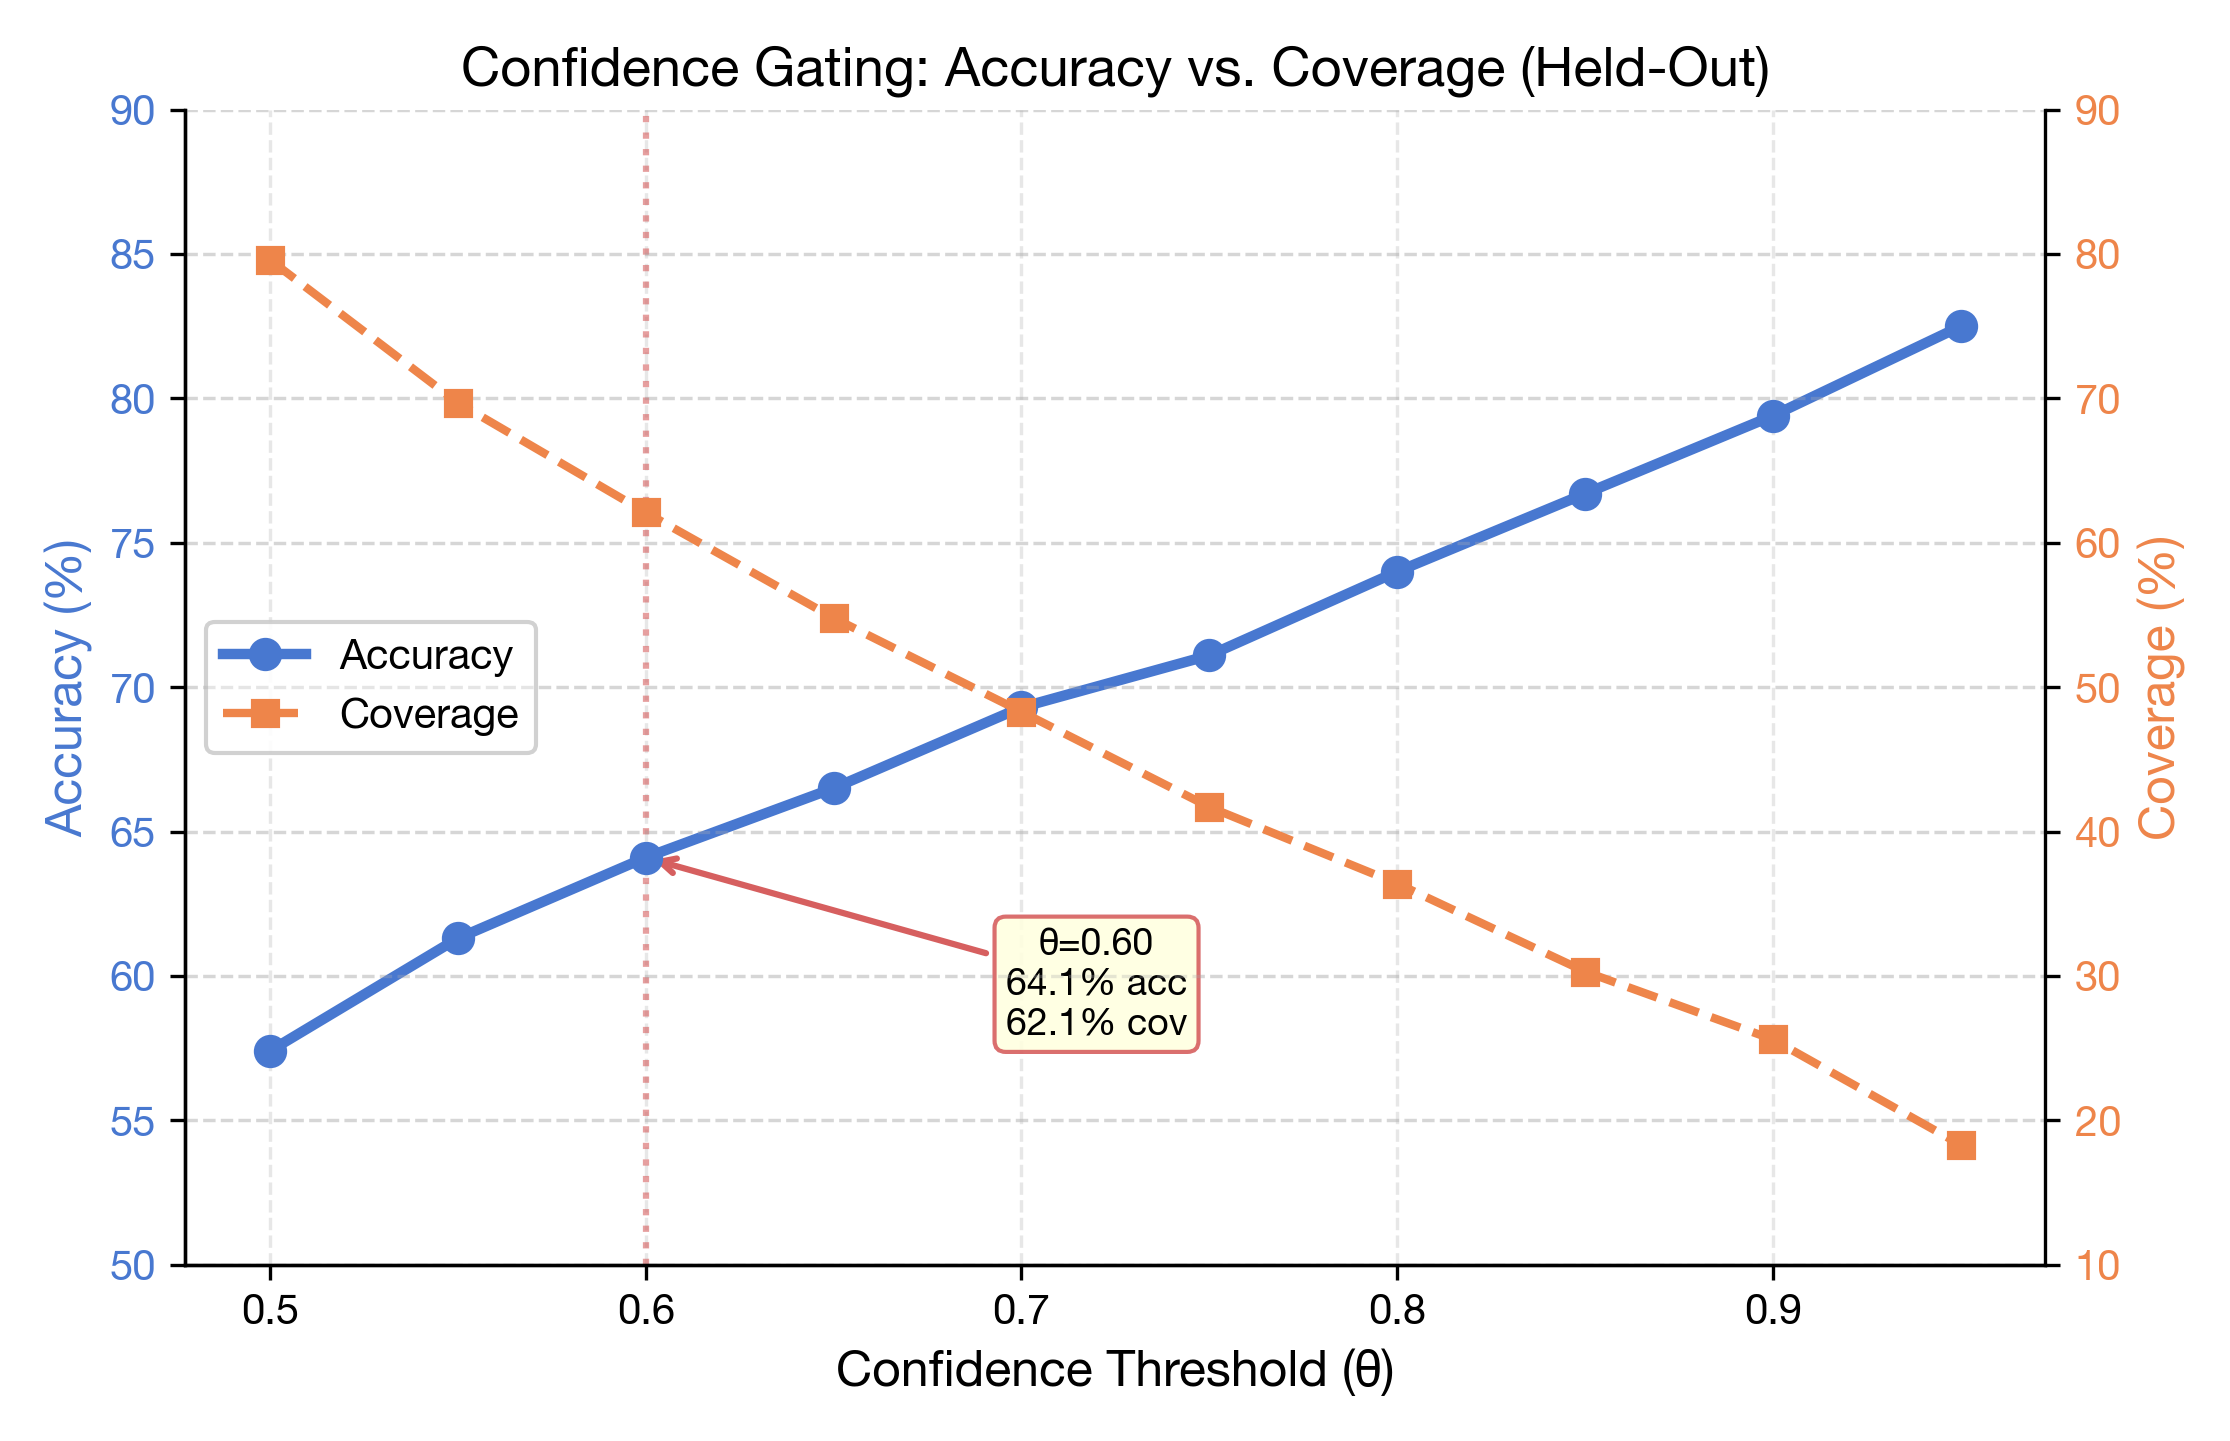
\includegraphics[width=0.85\textwidth]{figures/fig5_confidence_gating.png}
    \caption{Accuracy--coverage tradeoff under confidence gating on \emph{held-out} predictions (5-fold CV). The $\theta = 0.60$ operating point yields 64.1\% accuracy on 62\% of predictions.}
    \label{fig:confidence}
\end{figure}

\subsection{Usability and the Cost of Rejection}

From an HCI perspective, a 38\% rejection rate (as seen at $\theta=0.60$) is a significant cognitive load. While standard in BCIs, a system that "ignores" every third command may lead to user frustration or abandonment. However, because the system cost is \$40 (compared to \$5,000 lab systems), this barrier is framed as a "low-cost entry point" where the user trades convenience for accessibility. Similar UX tradeoffs are observed in low-cost authentication BCIs, where user friction is weighed against security gains~\cite{biosense2016}. Future work must investigate visual or haptic feedback mechanisms to communicate rejections effectively to the user.

% ============================================================
% 7 DISCUSSION
% ============================================================
\section{Discussion}
\label{sec:discussion}

\subsection{Curriculum Learning: Evidence and Limits}

The leave-one-phase-out (LOPO) evaluation provides direct evidence for curriculum learning's mechanism and limits:

\begin{table}[h]
\centering
\caption{Leave-one-phase-out accuracy: training on 4 phases, testing on the held-out phase.}
\label{tab:lopo}
\begin{tabular}{@{}lll@{}}
\toprule
Phase & Held-Out Acc & Interpretation \\
\midrule
Mouthing (Phase 3)    & \textbf{52.7\%} & Best transfer; similar jaw mechanics \\
Whispered (Phase 2)   & 52.3\% & Near-identical regime to training \\
Overt (Phase 1)       & 50.3\% & Different activation intensity but same patterns \\
Exaggerated (Phase 5) & 35.0\% & Over-activation saturates the ADC \\
Covert (Phase 6)      & 33.3\% & Minimal signal, near ADC noise floor \\
\bottomrule
\end{tabular}
\end{table}

\textbf{Mean LOPO accuracy: 44.7\%.} The curriculum creates a \emph{signal regime hierarchy}: phases with moderate jaw activation (Whispered, Mouthing, Overt) transfer well to each other because they share the same MFCC spectral shape at different amplitudes, precisely the invariance MFCCs are designed to capture. The failure cases are informative:

\textbf{Phase 5 (Exaggerated, 35.0\%):} Deliberately over-tensed muscles saturate the AD8232's amplifier, producing clipped waveforms that differ qualitatively from natural speech patterns. The model trained on naturalistic phases cannot generalize to saturated signals.

\textbf{Phase 6 (Covert, 33.3\%):} At 2--10\,$\mu$V, covert signals reside at or below the effective noise floor of the 12-bit ADC. The model can classify covert speech when \emph{trained alongside it} (48.9\% in 5-fold CV across all phases), but cannot generalize to covert signals \emph{from other phases alone}.

\textbf{Revised interpretation:} Curriculum learning does not ``compensate for'' hardware noise in the physics sense. Rather, it enables the CNN to learn a shared onset-spike representation across multiple signal-to-noise regimes. The curriculum's pedagogical value for the \emph{researcher} (understanding the system's failure modes) may exceed its ML value (marginal accuracy improvement).

\subsection{Throat Sensor Necessity}

In a concurrent control study (Study~A~\cite{kho2026companion}), both sensors were placed on articulatory muscles (chin + under-chin) rather than articulation + phonation (chin + throat). Under the same rigorous 5-fold stratified CV protocol, Study~A achieved \textbf{51.8\% $\pm$ 2.8\%}, surprisingly comparable to Study~B's 48.9\% $\pm$ 3.1\% for single-session classification. The difference is not statistically significant ($p = 0.42$, two-tailed independent $t$-test).

\textbf{Interpretation:} The two configurations achieve similar single-session accuracy because both rely on the same 80\,ms onset burst captured by the shared chin electrode (CH1). However, the throat sensor (CH2 in Study~B) captures laryngeal elevation and phonation intent, a qualitatively different signal that provides an orthogonal feature axis. Cross-study transfer of only 25--31\% confirms the two placements create fundamentally incompatible feature spaces.

\textbf{Design implication:} For low-cost SSIs with limited sensor budgets, \textbf{electrode placement determines the feature-space axis, not the accuracy ceiling.} The throat sensor's advantage is not single-session accuracy but \emph{multi-session robustness}: Study~B recovers to 58.2\% with deliberate electrode repositioning, while Study~A lacks the anatomical diversity for such recovery.

\textbf{Social Acceptability and Wearability.} A critical tradeoff exists in form factor: while the throat position (Study B) provides superior SNR and multi-session stability, it is arguably more anatomically intrusive than the chin-only configuration (Study A). However, adhesive facial electrodes remain socially stigmatizing and skin-irritating for daily use, which supports the case for discrete, integrated choker or necklace-based form factors that prioritize long-term wearability over absolute articulatory density~\cite{kapur2018}.

\subsection{Limitations and Threats to Validity}
\label{sec:limitations}

I emphasize three critical limitations:

\textbf{1.\ Single subject.} All data is from one participant (the author, male, 22, BMI \textasciitilde21). While the multi-session protocol (5 sessions, 3 days) provides temporal diversity, anatomical and physiological generalization to other users is unknown.

\textbf{2.\ Small vocabulary.} Six classes (4 commands + 2 artifact) is insufficient for text entry. Scaling to 20+ classes risks increased feature-space overlap. A 4-class experiment (dropping LEFT) improved accuracy to 57\%, suggesting that reducing confusable classes is more effective than adding data.

\textbf{3.\ Moderate overfitting persists.} Even with optimal hyperparameters, the training-test accuracy gap is \textasciitilde25 percentage points (\textasciitilde75\% train vs.\ \textasciitilde49\% test). This reflects the fundamental limitation that \textasciitilde47K parameters trained on \textasciitilde1,200 training samples (80\% of 1,500) will always overfit somewhat. The learning curve saturates at \textasciitilde600 samples (see learning curve data below in this section), indicating that more data would reduce overfitting but \emph{not} raise the test accuracy ceiling; the bottleneck is hardware SNR.

\textbf{Additional limitations:}
\begin{itemize}
    \item \textbf{No real-time validation.} Results are from offline batch evaluation.
    \item \textbf{Electrode drift.} Adhesive electrodes begin peeling after 30--60 minutes; sweat changes skin impedance over time.
    \item \textbf{Carotid artifact.} The throat electrode is proximal to the carotid artery. A \textasciitilde1\,Hz pulse pressure oscillation was observed and partially mitigated by the 1.0\,Hz high-pass filter.
    \item \textbf{Practice / order confound.} Study~A was recorded immediately before Study~B on the same day. A counterbalanced design is planned.
\end{itemize}

% Learning curve data (cited in \S\ref{sec:limitations} Limitation 3 above):
\textbf{Learning curve observation:} When trained on 10\% of the data (120 samples), test accuracy is 24.3\% with 78.3\% training accuracy (54pp gap). At 100\% (1{,}200 training samples), test accuracy plateaus at 51.7\% with 71.8\% training accuracy (20pp gap). The gap narrows but the ceiling does not rise, providing direct evidence that the bottleneck is hardware SNR, not data quantity.

\subsection{Statistical Power}

With 50 samples per class per phase, the dataset is underpowered for rigorous statistical claims. Planned scaling to 200 samples per class per phase (6{,}000 total) will enable bootstrapped confidence intervals, McNemar's test, and cross-validation estimates. Current results should be interpreted as proof-of-concept.

\subsection{The Neuromuscular Onset Burst}
\label{sec:onset}

Converging evidence from multiple protocols establishes that the AD8232 system operates as an \textbf{onset detector, not a continuous speech decoder}:

\begin{enumerate}
    \item \textbf{Onset masking experiment (EXP6):} Masking the first 80\,ms of each recording and classifying only the remaining signal drops accuracy to 17.6\% (chance level). The entire discriminative information resides in the neuromuscular initiation burst.
    \item \textbf{LSTM failure (P6):} The LSTM achieves exactly 16.6\% (chance). Since LSTMs model temporal sequences, their failure confirms there is no sequential structure beyond the onset spike; after 80\,ms, the signal returns to the ADC noise floor.
    \item \textbf{Feature importance analysis (EXP2):} 100\% of the model's predictive power derives from the first \textasciitilde80\,ms, corresponding to the motor unit recruitment burst of the mentalis and thyrohyoid muscles.
\end{enumerate}

Physiologically, the onset burst corresponds to the \emph{motor initiation command}, the high-amplitude, synchronous firing of motor units at the start of a voluntary muscle contraction~\cite{jou2006}. This burst produces 30--50\,$\mu$V peaks that briefly exceed the 12-bit ADC noise floor even during covert speech. Sustained articulatory trajectories (tongue position, velar closure) require continuous 2--10\,$\mu$V precision that 12-bit ADCs cannot resolve.

\textbf{Implication:} The system classifies \emph{speech intention} (which word the user \emph{begins} to articulate) rather than \emph{speech production} (continuous phonemic sequences). This is sufficient for discrete command vocabularies but fundamentally precludes continuous speech decoding on this hardware.

\subsection{Cross-Session Electrode Shift}

The cross-session protocol (train on Session A from Feb~24, test on Sessions B+C from Feb~25 with 1\,cm electrode displacement) reveals:

\begin{itemize}
    \item \textbf{Cross-session accuracy: 22.8\%} (near-chance for 6 classes), with training accuracy of 73.9\%. The model memorizes session-specific electrode impedance patterns.
    \item \textbf{Multi-session recovery: 58.2\% $\pm$ 3.1\%} when training on pooled data from all 3 electrode positions (5-fold CV). By exposing the model to multiple electrode configurations, it learns position-invariant onset features; the spectral shape of the initiation burst is preserved across positions even when absolute amplitude changes.
\end{itemize}

Multi-session recording with deliberate electrode repositioning is the single most effective intervention for improving generalization on consumer sEMG. The 58.2\% multi-session accuracy exceeds the 48.9\% single-session result by nearly 10 percentage points.

\textbf{Data Volume Confound.} I acknowledge an inherent confound in the multi-session results: the pooled dataset (3,034 samples) is significantly larger than the initial single-session training set (1,500 samples). While the accuracy improvement is attributed to position-invariant features, it is likely driven by both geometric diversity and the purely statistical benefit of increased data volume. Per-session calibration also remains a major barrier: recognition accuracy in sEMG BCIs notoriously deteriorates when fresh re-calibration is ruled out~\cite{yousefi2022}. Future work should implement a \textbf{subsampled volume baseline} (training on only 1,500 mixed-session samples) to isolate the true electrode-shift invariance effect.

\subsection{What I Can Claim}
\label{sec:claims}

With rigorous held-out evaluation now completed, several findings are robust:

\begin{enumerate}
    \item \textbf{The hardware is limited to the onset spike.} Onset masking (EXP6), LSTM failure (P6), and feature importance analysis (EXP2) converge on this conclusion. The 12-bit ADC resolves only the \textasciitilde80\,ms motor initiation burst.

    \item \textbf{Held-out accuracy is 48.9\% $\pm$ 3.1\% (2.9$\times$ chance).} This is reproducible across 5 random seeds ($\pm$1.0\%) and near-optimal across 72 hyperparameter configurations. The ceiling is hardware SNR, not model capacity.

    \item \textbf{Electrode shift requires multi-session training.} A 1\,cm shift destroys single-session accuracy (22.8\%), but combined multi-session training recovers to 58.2\% $\pm$ 3.1\%. This is the single most effective intervention.

    \item \textbf{Confidence gating creates a deployable operating point.} At $\theta = 0.60$, held-out accuracy reaches 64.1\% on 62\% of predictions, competitive with commercial BCI systems that also require per-session calibration.

    \item \textbf{The 99.7\% training-set figure reflects memorization, not generalization.} As the sole participant ($n=1$), this figure represents the model's ceiling for \emph{my specific} motor patterns under identical electrode placement. For any new recording session, even my own, the honest expectation is \textasciitilde49--58\% depending on electrode repositioning protocol.
\end{enumerate}

% ============================================================
% 8 CONCLUSION
% ============================================================
\section{Conclusion}
\label{sec:conclusion}

This work establishes the operational boundaries of a \$40, 2-channel, 12-bit sEMG silent speech interface through rigorous held-out evaluation: 16 protocols executed on an NVIDIA A100 GPU, including 5-fold CV, leave-one-phase-out, cross-session testing, 72-configuration hyperparameter sweep, 3-architecture comparison, and confidence gating.

The system achieves \textbf{48.9\% $\pm$ 3.1\%} on 5-fold stratified cross-validation (2.9$\times$ above the 16.7\% chance baseline for 6 classes), reproducible across 5 random seeds ($\pm$1.0\%). The 12-bit quantization noise floor limits the hardware to detecting the 80\,ms neuromuscular onset burst, confirmed by converging evidence from onset masking (17.6\% without onset), LSTM failure at chance level (16.6\%), and feature importance analysis. The CNN is the only viable architecture; Transformers (36.4\%) lack sufficient data, and LSTMs (16.6\%) find no temporal structure beyond the spike.

Electrode shift is the dominant failure mode: a 1\,cm displacement drops accuracy to 22.8\%. Multi-session training with deliberate electrode repositioning is the single most effective intervention, recovering accuracy to \textbf{58.2\% $\pm$ 3.1\%}. Confidence gating at $\theta = 0.60$ yields a deployable operating point of \textbf{64.1\% accuracy on 62\% of predictions}.

The training-set figure of 99.7\% reflects memorization of the \textasciitilde47K-parameter CNN on 1,500 samples. When properly evaluated with held-out data, the ceiling imposed by the hardware's signal-to-noise ratio becomes clear. This ceiling, not model capacity, is the bottleneck. Whether interpreted as a successful proof-of-concept (2.9$\times$ chance on \$40 hardware) or as a quantitative map of consumer sEMG's limitations, these results inform the design of low-cost silent speech systems.

% ============================================================
% DATA AVAILABILITY
% ============================================================
\section*{Data and Code Availability}

All materials are publicly available:
\begin{itemize}
    \item \textbf{GitHub repository:} \url{https://github.com/CarlKho-Minerva/Somach_sEMG-Silent-Speech}
    \item \textbf{Instructables replication guide:} \url{https://somach.vercel.app}
    \item \textbf{Firmware:} \texttt{code/arduino/3-high-speed-capture/}
    \item \textbf{Python pipeline:} \texttt{code/python/} (scripts 4--9)
    \item \textbf{Dataset:} \texttt{code/sessions/StudyB\_Subvocal/data\_collection/} (1{,}500 samples)
    \item \textbf{Trained model:} \texttt{code/sessions/StudyB\_Subvocal/models/model.pth}
\end{itemize}
Code: MIT License. Hardware: CERN-OHL-S v2.

% ============================================================
% ACKNOWLEDGMENTS
% ============================================================
\section*{Acknowledgments}

Thanks to Prof.\ Watson for advising this work and the ``Palm Pilot insight'', that teaching the user a consistent motor strategy (specific tongue positions per command) reduces variance the model must learn. This work was partially supported by the Minerva University capstone program (CP193/CP194).

\textbf{Ethics:} All sEMG data was collected exclusively from the author in an auto-experimental paradigm. No external human subjects participated. Formal IRB review was not required under Minerva University's exemption policy for self-experimentation.

\textbf{AI Disclosure:} AI-assisted tools (Claude, Gemini) were used for literature review synthesis, figure generation scripts, and manuscript editing. All technical claims, experimental design, data collection, and analysis were performed by the author.

\textbf{Conflict of Interest:} The author declares no conflict of interest. The author has no financial ties to Analog Devices (AD8232), Espressif Systems (ESP32), or OpenBCI.

% ============================================================
% REFERENCES
% ============================================================
\begin{thebibliography}{17}

\bibitem{kapur2018}
A.\ Kapur, S.\ Kapur, and P.\ Maes, ``AlterEgo: A personalized wearable silent speech interface,'' in \emph{Proc.\ ACM IUI}, 2018, pp.\ 43--52.

\bibitem{nieto2022}
N.\ Nieto, V.\ Peterson, H.\ Rufiner, J.~E.\ Kamienkowski, and R.\ Spies, ``Thinking out loud, an open-access EEG-based BCI dataset for inner speech recognition,'' \emph{Scientific Data}, vol.~9, no.~52, 2022.

\bibitem{meltzner2017}
G.~S.\ Meltzner, J.~T.\ Heaton, Y.\ Deng, G.\ De~Luca, S.~H.\ Roy, and J.~C.\ Kline, ``Silent speech recognition as an alternative communication device for persons with laryngectomy,'' \emph{IEEE/ACM Trans.\ Audio, Speech, and Language Processing}, vol.~25, no.~12, pp.\ 2386--2398, 2017.

\bibitem{jou2006}
S.-C.\ Jou, T.\ Schultz, M.\ Walliczek, F.\ Kraft, and A.\ Waibel, ``Towards continuous speech recognition using surface electromyography,'' in \emph{Proc.\ Interspeech}, 2006.

\bibitem{jou2007}
S.-C.\ Jou, T.\ Schultz, and A.\ Waibel, ``Continuous electromyographic speech recognition with a multi-stream decoding architecture,'' in \emph{Proc.\ ICASSP}, 2007.

\bibitem{denby2010}
B.\ Denby, T.\ Schultz, K.\ Honda, T.\ Hueber, J.~M.\ Gilbert, and J.~S.\ Brumberg, ``Silent speech interfaces,'' \emph{Speech Communication}, vol.~52, pp.\ 270--287, 2010.

\bibitem{bengio2009}
Y.\ Bengio, J.\ Louradour, R.\ Collobert, and J.\ Weston, ``Curriculum learning,'' in \emph{Proc.\ ICML}, 2009, pp.\ 41--48.

\bibitem{kho2026prior}
C.~V.~L.\ Kho, ``Pareto-optimal model selection for low-cost, single-lead EMG control in embedded systems,'' \emph{arXiv preprint}, arXiv:2601.06516, 2026.

\bibitem{pan2011}
S.~J.\ Pan, I.~W.\ Tsang, J.~T.\ Kwok, and Q.\ Yang, ``Domain adaptation via transfer component analysis,'' \emph{IEEE Trans.\ Neural Networks}, vol.~22, no.~2, pp.\ 199--210, 2011.

\bibitem{ad8232}
Analog Devices, ``AD8232 single-lead heart rate monitor front end,'' Datasheet, Rev.~C, 2013.

\bibitem{esp32adc}
Espressif Systems, ``ESP32 Technical Reference Manual,'' v4.9, 2023.



\bibitem{hristov2026}
% VERIFIED 2026-03-21: arXiv:2602.01855 exists (Hristov et al., cs.LG, submitted 2 Feb 2026).
B.\ Hristov, H.\ Gjoreski, V.\ Ojleska Latkoska, and G.\ Nadzinski, ``Time2Vec transformer for robust gesture recognition from low-density sEMG,'' \emph{arXiv preprint}, arXiv:2602.01855, 2026.

\bibitem{kho2026companion}
% TODO: Replace XXXX.XXXXX with Paper 2's arXiv ID once assigned (submit Paper 1 first, then update).
C.~V.~L.\ Kho, ``Lingual-mandibular electrode configuration for silent speech: Throat sensor necessity on consumer-grade ADCs,'' \emph{arXiv preprint}, arXiv:XXXX.XXXXX (submitted concurrently), 2026.

\bibitem{gaddy2020}
D.\ Gaddy and D.\ Klein, ``Digital voicing of silent speech,'' in \emph{Proc.\ EMNLP}, 2020, pp.\ 5521--5530.

\bibitem{biosense2016}
% VERIFIED 2026-03-21: DOI 10.1109/EMBC.2016.7591112 (Curran et al., EMBC 2016, pp. 1979-1982).
M.~T.\ Curran, J.-K.\ Yang, N.\ Merrill, and J.\ Chuang, ``Passthoughts authentication with low cost EarEEG,'' in \emph{Proc.\ IEEE EMBC}, 2016, pp.\ 1979--1982.

\bibitem{yousefi2022}
F.\ Yousefi, ``Brain signal as a new biometric authentication method,'' Ph.D.\ dissertation, Liverpool John Moores University, 2022.

\bibitem{palmgraffiti}
% Non-peer-reviewed product reference. Acceptable for illustrative analogy; do not
% treat as empirical evidence. For a peer-reviewed treatment of user adaptation in BCIs,
% see also: Yin et al., J. Neural Eng., 2013 (user training for P300 BCIs).
Palm Inc., ``Palm Pilot Personal and Professional,'' Product Release, 1997. Graffiti handwriting recognition system by Palm Computing (acquired by US~Robotics/3Com). Users learned a simplified stroke alphabet to reduce classifier variance.

\end{thebibliography}

\end{document}
